%\section{Introduction}
\label{sec:evaluation:introduction}

The evaluation of corpus construction is a particularly tricky area: without a gold standard or real-world task to frame the results, it is often difficult to tell quantitatively what differences between corpora constitute improvements.


The way seed-based methods work offers an ideal source of gold standard data, nonetheless, only experience and repeated use can reveal the manner of the differences identified, and its impact on experimental results.  This evaluation will use this reflexive method to identify overall responsiveness to the seed corpus, along with an examination of individual components of the system as a method for revealing specific strengths and weaknesses.

This evaluation is based around one of tasks identified in Chapter~\ref{sec:rebuilding}---that of rebuilding a corpus from scratch based upon a seed's proportions.  This task is effectively a super-task of reconstructing or repairing a corpus, and is equivalent to many scenarios involving disseminating sensitive corpora with minor restrictions on the metadata dimensions used.



This chapter begins with a description of the use cases covered, and a detailed rationale of how these form testable, objective research questions.

Section~\ref{sec:evaluation:rqs} details the two main approaches to evaluation: those applied to individual components, and those applied to the results of running the implementation as a whole.

Following that, each stage of the corpus building process is evaluated in a white-box fashion, starting with the heuristics used to classify documents (Section~\ref{sec:evaluation:heuristics}) and moving on to the process of identifying `target' prototype documents in vector space (Section~\ref{sec:evaluation:resampler}), and then retrieving documents from the web itself (Section~\ref{sec:evaluation:retrieval}).

Finally, the implications of each component's functionality to the final process, and what the results tell us about the state of the web as a document source for resampling BNC-like corpora, are discussed in Section~\ref{sec:evaluation:discussion}.







\section{Evaluation Criteria}
\label{sec:evaluation:rqs}


The overall method used in this evaluation is one of treating the system to be tested as a method of replicating the features of a corpus, passing statistical properties of the input corpus through to the output.

The capacity of any system using auxiliary data to do this is dependent on the nature of the population, and how it relates to the input.  The data used for evaluation must then be a subset of the population of documents accessible using the search heuristics chosen---if testing with another seed corpus, one must change the search strategy modules to fit, changing the overall results of the tool.  Essentially, this is a manifestation of 'garbage in, garbage out': moving search strategies into the implementation merely makes this more explicit.

One method of testing this is to see the output corpus as a model of the input, given certain assumptions that include the selection of metadata types and search strategies: providing those assumptions hold, much of the variation in the input corpus ought to be explained by variation in the output.  Measuring deviance between the two allows us to identify specific areas of poor fit, which can then be improved either by altering the pluggable modules to fit the ground truth.

The purpose of this evaluation is to test both the search modules used for the particular corpora given, and the overall method: if no set of reasonable assumptions can be found, this is an indication either that the population of documents online is fundamentally different to that of the input corpora tested, or the method presented here is incapable \textsl{by design} of identifying appropriate documents.

% --

Research questions surrounding this method run to:

\begin{itemizeTitle}

    \item[Components] How valid are the assumptions of each of the retrieval methods and heuristics selected?

    \item[Overall Application] For general-purpose input corpora, to what extent (and in what manner) does the output corpus resemble the input `seed' corpus?

    \item[Feature Correlation] Do the differences between two input corpora match those between two corpora built using them as seeds?

    \item[Residual Variance] What consistent features remain variable between the output and input corpora, i.e. what data cannot be sought online using the heuristics/search methods selected.

\end{itemizeTitle}

The accuracy of each heuristic component is constributory to the excess dispersion in the output corpus.  By design these modules are unambitious, relying on existing methods and tools already tested in the literature, however, their performance upon the data used here will be evaluated in order to better explain sources of error.  As this system remains a proof of concept, the selection of these modules is limited.






\til{put in discussion: this restriction already exists for tools like bootcat, but without the explicit control over search mechanisms provided using the method being evaluated here.  Since there is no theoretical way around the `garbage in garbage out' problem, providing easy operationalisation to users is one approach to reducing overall methodological errors}

---notably, selecting a wildly different input corpus without changing the sources of data will result in wildly different 







\section{Performance of Heuristics}
\label{sec:evaluation:heuristics}
The heuristics selected for this evaluation are formed around Lee's BNC World index~\cite{lee2003bnc}.  This selection was chosen because of their alignment to operationalisable, human-level metadata and the existence of multiple corpora with this level of annotation.



There are two main approaches to populating the corpus description using these heuristics: either read the seed corpus' contents and classify each data point, or read a list of metadata from an existing index.  The latter approach is used in this evaluation, since it is applicable to corpora with partially-missing data (such as the personal corpus data resulting from data gathering in Chapter~\ref{5}).

The accuracy of the classifiers listed here is responsible for minimising excess dispersion relative to the input corpus.  The nature of their residual error is also going to apply bias to the resulting data set.

Since many of these heuristics surround operationalising a corpus, a large body of research exists for classifying and extracting useful dimensions from texts.  The heuristics presented here are proof-of-concept only, and it is expected that the design of the heuristics used for a study is selected to match the theoretical basis of any analysis.

The heuristics presented here are document-level.  In most corpus designs, word count would be considered a measure of the size of the corpus (rather than a property of its constituents).  The method evaluated here is capable of retrieving truly IID\td{elaborate} samples at different levels, and demands a different selection of heuristics and metadata when operating at the word or sentence level.  Document level metadata are both high-level enough to be distributed for confidential corpora and descriptive enough to enable accurate retrieval (by contrast, word or part-of-speech frequencies would reveal much of the contents of the original corpus, which may not be desirable).




\subsection{Audience Level}
The BNC User's Reference Guide~\cite{CITE} describes audience level thus:

\begin{quote}
...a subjective assessment of the text's technicality or difficulty.
\end{quote}

This is expanded upon slightly by Lee~\cite{lee2003bnc}, saying:

\begin{quote}
    \textsl{Audience level}, on the other hand, is an \textbf{estimate} (by the compilers) of the \textbf{level of difficulty} of the text, or the amount of background knowledge of its subject matter which is assumed.
\end{quote}

One approach to modelling this complexity is to use word lists such as those used in education, however, this is difficult to apply to such disparate topics without extensive compilation of such lists.  A simpler approach uses metrics computed from the morphology of words to form a readability score.  Such metrics are already widely used in word processing software and for designing documents for public consumption.


The classifier used for evaluation is based on the Flesch reading ease score~\cite{flesch1948new}.  This score is widely used, easy to compute, and correlates with the simple `low/med/high' classification used in the BNC metadata:

$$
readability_{F} = 06.835 - 1.015 \left( \frac{\text{total words}}{\text{total sentences}} \right) - 84.6 \left( \frac{\text{total syllables}}{\text{total words}} \right)
$$


%Readability ranks: 
% - med: 1651 items, mean = 55.44412267430666, sd = 12.76812426643693, var = 163.02499728317557
% - low: 664 items, mean = 62.95293871760397, sd = 14.424512199650604, var = 208.06655219786907
% - high: 820 items, mean = 47.70965585209567, sd = 12.445956325065204, var = 154.90182884543054
% - ---: 914 items, mean = 82.02288020623476, sd = 20.6424573733852, var = 426.111046412025
%Classifier error: 
% - med: 1239 / 1651 = (75.04542701393095%
% - low: 226 / 664 = (34.036144578313255%
% - high: 277 / 820 = (33.78048780487805%
% - ---: 914 / 914 = (100.0%
\begin{table}[h]
    \center
    \begin{tabular}{|c|c|c|c|}
        \hline 
        $\bar{readability_{F}}$ & BNC Audience level & Standard Deviation & na\"ive acc. \\
        \hline 
        63 & Low & 14.4 & 65.9\% \\
        55 & Med & 12.7 & 25.0\% \\
        47 & High & 12.4 & 66.3\% \\
        82 & (unclassified, speech) & 20.6 & - \\
        \hline
    \end{tabular}
    \caption{Target Flesch reading ease scores and their equivalent BNC categorisation.}
    \label{tab:evaluation:heuristics:fscore}
\end{table}




%plot(density(as.numeric(as.character(dat$readability))), main="BNC World Flesch-Kincaid Readability Scores", xlab="Readability Score (bandwidth: 3.192)")

In order to establish the meaning of the BNC audience level categories in terms of this score, means were computed from the BNC world data.  These means, shown in Table~\ref{tab:evaluation:heuristics:fscore} (a reproduction of Table~\ref{tab:rebuilding:method:fscore}), were used by a simple classification algorithm that selects the category with the nearest mean value.  This na\"ive method yields the accuracy indicated in the `na\"ive acc.' column of Table~\ref{tab:evaluation:heuristics:fscore}, indicating that the readability score is not an ideal measure of the audience level.



\begin{figure}[h]
    \centering
    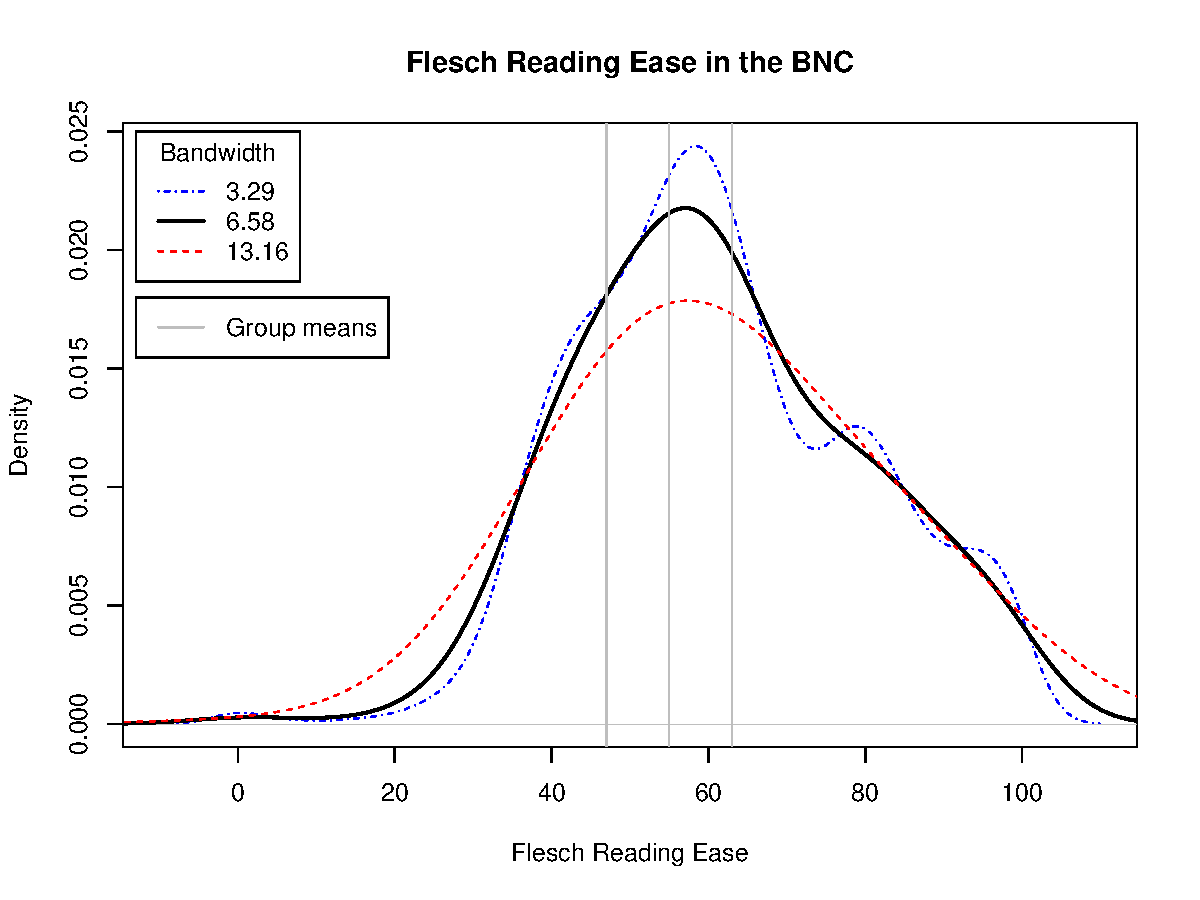
\includegraphics[width=0.8\textwidth]{evaluation/fleschbncdist}
    \caption{Flesch reading ease distribution in the BNC.}
    \label{fig:evaluation:heuristics:fleschbncdist}
\end{figure}


Rather than continue to use the categorisation used in the BNC, each text was scored for readability and the raw Flesch reading ease score used as its point within that dimension.  The `cpr' profiling tool then simply represents the underlying distribution as a continuous one (rather than artificially discretised into `high', `medium' and `low').

The standard deviation of categories within Table~\ref{tab:evaluation:heuristics:fscore} provides us with a convenient source for the bandwidth of the smoothing function used to identify the empirical distribution of the reading ease scores.  Using graphical methods (illustrated in Figure~\ref{fig:evaluation:heuristics:fleschbncdist} the value of $\sigma / 2$ was chosen to represent the distribution: this offers a tradeoff between accurately portraying the distribution and permissively selecting documents online.  This method also clarifies the difficulties associated with attempting to accurately classify audience level based on readability metrics.

Where a text is unavailable, knowledge of the standard deviation of each of the readability categories in the BNC allows us to produce an approximation of the distribution of readability scores.  This approach (as well as the smoothing above) illustrate the value of manually modifying the text distributions during the design phase.

As we are using a proxy variable to impute the reading ease, any classifier accuracy issues are deferred to the assumption that `reading ease' is something we, as corpus designers, care about.






\subsection{Word Count}
Word counts are, for our purposes, trivial to compute.  There are two challenges to operationalising word counts, however.

The former of these pertains to metadata and other boilerplate within files.  Files must be processed prior to word counts being performed.  This means (like many other tools) that we must post-process candidate files even if we elect to discard their contents.

Secondly, it is necessary to normalise deviance measures when comparison documents: this poses a particular challenge as word counts are open-ended.  The method used here was to enforce an arbitrary limit, above which any distances in the word count dimension register as $1$.  Because the sampling method does not primarily rely on gradient descent, this is fairly safe, however, selection of the threshold does impact the importance assigned to word count (vs. some other metadata dimension): too high and it will undervalue differences in word count.

The arbitrarly limit selected for the BNC was \td{limit from config file}.  This is sufficiently large that it encompasses the word counts for all BNC files, allowing for at least \td{n\%} excess.  In practice (as we shall discuss later~\td{where}) most documents fall short, and this limit could be reduced.

% --- 
It is worth noting the difference in philosophy this method embodies compared to many corpus studies: the word count here is a property of each document, and not a measure of corpus size.  Unlike many methods, we are sampling at the same level we are presuming analysis at (though this level is variable due to the ease with which documents may be selected).






\subsection{Genre}
Genre is arguably the most important single stratification applied to a general-purpose corpus (even forming the bulk of the definition of its name), yet it remains one of the more nebulous terms.  Here we follow Lee's definitions once more, commensurate with the BNC index that serves as the source of much of the metadata for our corpus definition file.

Due to the complexity of genre taxonomies (and thus the relative difficulty of classifying documents therein), there is significant motive to take the same approach as audience level above: using a self-defined or simpler taxonomy to simplify imputation or selection.  On the other hand, the BNC classification is well-known and likely to be used in any corpus augmentation task (``I want this subset of the BNC, but \textsl{more} of it.'').  We describe here an approach using the existing BNC classifications for this reason, with a detailed discussion of the implications of other options below\td{where}.


As this is a proof-of-concept system, the accuracy of the classifiers used need not be cutting-edge.  This relaxed requirement is reinforced by the notion that any errors are `sane', falling along such ambiguities as identified by Lee~\cite[p.~11]{lee2003bnc}:

\begin{quote}
It may be the case that the actual content/topic of these linguistics-related texts makes them seem less like social science texts than arts or applied science texts...
\end{quote}

This `sanity of error' is enforced by using a distance measure that is based on rank correlation of token type frequencies, allowing two categories to be judged on a scale more meaningful than simple boolean equality.  This luxury may not be available for all potential discrete classification systems (such as those read from external indices), and is not a requirement of convergeance to the input distribution.

The distinction between genres is often somewhat variable: some, such as \variable{w\_newsp\_brdsht\_nat\_*}, are made between the subject of texts, whereas others fall along lines of context or what others may term `text type' (\variable{W\_email} vs. \variable{W\_essay\_sch}).  This makes it particularly difficult to identify a model that linearises features within the dataset consistently enough for many classification algorithms to work well.

Lee's taxonomy is partially hierarchical, with many of the more detailed categories harbouring both this `text type' distinction as well as one regarding topic.  Both were retained here as they align to two distinct processes when sampling: the text type is an indication of (roughly) where a document may be found, and the topic regards more which document to select.





% --

\paragraph{}
The problem of identifying BNC genre from free text is a simple 70-way classification task\footnote{Such that a 70-way classification task may be described as simple at all.}.  In practice, the subjective nature of the taxonomy and the large number of classes makes this a challenging endeavour.  This is a clear illustration of the difficulties encountered using the ImputeCaT method: whilst it may not be necessary to find documents online with great accuracy, there must exist \textsl{some} method of discriminating between them in a useful way.



In his 2007 paper on web genres, Sharoff~\cite[p. 5]{sharoff2007classifying} fits a number of classifiers to the BNC, using a variety of genre taxonomies.  Therein he reports success using a supervised learning approach to classify `grouped' versions of the BNC taxonomy: one aligned to the EAGLES~\cite{EagTcwgCtypeaglespreliminary} text typology recommendations, and one 10-way grouping based on unsupervised methods.

\til{Mention Biber et. al, perhaps}

Since part of the intent here is to retain a parsimonious corpus profile document, this heuristic makes use of the original categories from the BNC taxonomy.  Nonetheless, Sharoff's study was used as a starting point for the methodology, in line with the goal of using established methods for heuristics.

The ambiguity and external nature of some of the distinctions drawn in the BNC index causes problems here, and represents a common dichotomy in linguistics: a human-readable and intuitive classification is not necessarily easy to model (to the point where we are often simply unable).

Ultimately, the classifiers detailed here used the na\"ive Bayes approach and were fit using WEKA~\cite{hall2009weka}.  In accordance with the findings of McCallum \& Nigam, the multinomial model was used over the Bernoulli due to its ability to maintain classification accuracy in models with large numbers of dimensions~\cite{mccallum1998comparison} (this also unexpectedly yielded the benefit that it was much faster to fit).

For the use-case presented here, absolute accuracy of the classifier matters little: we care only that `positive'ly classified cases are reliable for any one pass over the set of candidate documents, not that every candidate is selected.  Because of this, and because the number of classes is high enough to indicate that errors are unlikely to occur in the direction of the current class, the evaluations below focus on the precision of each method.

As ever, the classifier performance reveals as much about the taxonomy of the input data as it does the classification method.  Presented here are four models that cover different subsets of the BNC:

\begin{itemizeTitle}
    \item[BNC70] A classifier built using all 70 categories of both written and spoken BNC portions.
    \item[BNC69a] This classifier omits \texttt{S\_conv}, which was deemed unreasonably general in its content and thus difficult to retrieve.
    \item[BNC69b] The BNC70 classifier, omitting \texttt{W\_misc} due to the breadth of said category.
    \item[BNC68] Omitting Both \texttt{W\_misc} and \texttt{S\_conv}.
    \item[BNC46] Written portions of the BNC, containing \texttt{W\_misc}.
    \item[BNC45] Written portions of the BNC, without \texttt{W\_misc}.
\end{itemizeTitle}

The decision to omit sections of the BNC was deemed a necessary trade-off to achieve functional performance: for the purposes of this evaluation, the actual subset used is only of importance to the generality of the results (rather than their veracity).  Likewise, the priority is not to produce a genre classifier, but merely to use one within the larger method: simply, it is more important that the classifier is functional than that it is general.

% Comparison of each model, with graphs.
\begin{table}[ht]
    \centering

    \begin{tabular}{ |l|c|c|c| }
        \hline 
        Corpus & Accuracy & Precision & AUC \\
        \hline
        BNC45  &  70.7\%  &  .721  &  .901 \\
        BNC46  &  63.7\%  &  .666  &  .877 \\
        BNC68  &  71.5\%  &  .715  &  .913 \\
        BNC69a &  65.9\%  &  .685  &  .893 \\
        BNC69b &  72.1\%  &  .732  &  .918 \\
        BNC70  &  66.6\%  &  .689  &  .899 \\
        \hline
    \end{tabular}
    \caption{Weighted mean performance (per class) for each classifier.}
    \label{table:evaluation:heuristics:classifieraccuracy}
\end{table}

\til{Comments on 45 and 46 were lost when the HDD went, but the models remain.  Comment below}

Table~\ref{table:evaluation:heuristics:classifieraccuracy} shows the resultant accuracy figures for the models trained on the BNC subsets mentioned.  10-way crossvalidation was used to estimate the above statistics, in an effort to reduce the potential for overfitting to a fixed test/training set.  The statistics are formed from a weighted mean of each classes performance against all others.

These figures reveal that {\textsl spoken conversation} ({\texttt{S\_conv}) has the most deleterious effect on classifier accuracy, indicating that it overlaps most with other categories.  Whilst it was expected that \texttt{W\_misc} would also do this, the performance improvement shown in BNC69b over BNC68 indicates that \texttt{W\_misc} contains some distinct features that are best retained.  Though using a different design of classifier, overall performance is roughly in-line with Sharoff's BNC-based classifiers\footnote{Notably, attempts to fit SVM-based models lead to lower performance than multinomial na\"ive Bayes.  I believe this to be a result of the high number of classes}~\cite[ibid.]{sharoff2007classifying}.
    

\begin{figure}[Ht]
    \centering
    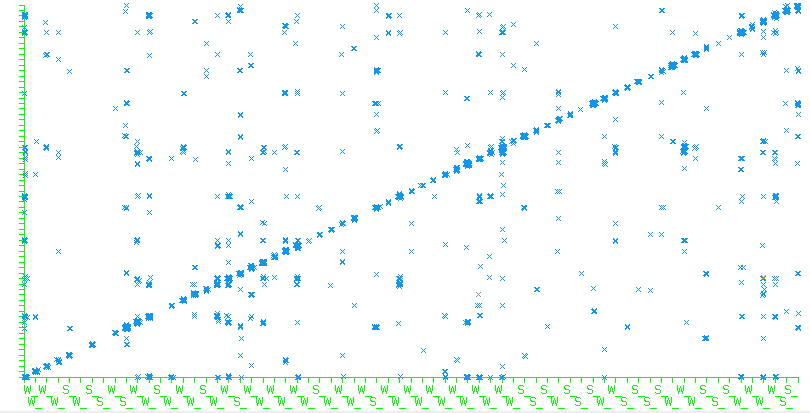
\includegraphics[width=1\textwidth]{evaluation/bnc68bconfusion}
    \caption{BNC68b confusion matrix}
    \label{fig:evaluation:heuristics:bnc68bconfusion}
\end{figure}



There are also potential arguments for the omission of many other categories from the taxonomy used here, however.  Figure~\ref{fig:evaluation:heuristics:bnc68bconfusion} shows the confusion matrix for the BNC69b classifier---note that some jitter has been applied to the plot to accentuate the overplotted items.  This shows a rough smattering of difficult-to-classify classes, though a more detailed inspection of the per-class tests on the model indicates that only two of these perform with AUC values below 0.7: \texttt{W\_fict\_drama} and \texttt{W\_essay\_univ}, which are classified in a way indistinguishable from chance.  Some classes with distinct lexical features (such as \texttt{W\_email} and \texttt{S\_sermon}) are classified particularly accurately.

The error surface described in Figure~\ref{fig:evaluation:heuristics:bnc68bconfusion} will contribute to the resulting error of the system, and as such further increase the variance of the output corpus.  Again, this is analogous to the coding stage of any conventional corpus building project, but with the distinct advantage that the propensity for classification error is well-known.

\til{ Insert the full accuracy data into an appendix and refer to it here }

% -- 
\paragraph{}

One final note should cover the generality of the methods used here.  As with all portions of the heuristics, the choice of classifier is heavily theory-laden, and should conform to the underlying data's nature as much as possible.  Classification of genre is a particularly awkward aspect since it relies on imputing fairly complex external information (such that it can then be worked with by the software) from linguistic content, something that, as a rule, should be avoided for the sake of statistical validity.  Notably, the EAGLES guidelines on text typology~\cite{EagTcwgCtypeaglespreliminary} warn:

\begin{quote}
The classification of texts into different genres seems to have been mostly achieved through external criteria rather than through internal, linguistic criteria.
\end{quote}

The manner of retrieval and the nature of the web offer some avenues for working with external data and closing this gap: It is firstly possible to retrieve documents according to an existing genre directory, all but guaranteeing a fit.  Further, HTML and HTTP metadata and stylistic properties of web documents (or those which are closely linked) may indicate genre as (or more) effectively as linguistic content.  These are all places where further research dovetails with the methods described here to increase overall accuracy.  Further work would be necessary to validate methods of reliably extracting and using this data, especially where it is patchy or difficult to extract.  Such efforts would prove particularly fruitful, however, where the seed corpus originates online, allowing the profiling and heuristic classification stages to operate using the same implementation.









\section{Performance of Resampling}
\label{sec:evaluation:resampler}

The accuracy of the resampling process depends lagely on two user-controlled properties:

\begin{itemize}
    \item The amount of smoothing applied to continuous metadata in the corpus.  Since values are selected from the smoothed corpus values, it is possible to select values that are non-identical to the input corpus.  This is generally a desirable property, and the kernel function used to smooth the input data is user-defined and has known statistical properties.
    \item The number of documents selected.  As this increases, the overall distribution of the output corpus converges to that of the corpus description file.
\end{itemize}


The intricacy of the input distribution largely defines the necessary size of the input corpus: an input corpus that is defined only in terms of simple marginal distributions is simpler to reproduce, that is it contains \textit{less information}, than one built using the full conditional distribution of a large, general corpus such as the BNC.

The question of when to stop sampling documents is related to the problem of corpus size in general: the output corpus is conceptually a model of the input corpus, and should contain enough data to be representative of the relationships therein whilst following the same guide.  This is best assessed by measuring the uniformity of residuals.  A suitable end condition for many uses of the output would thus be a combination of corpus size and residual uniformity (notably it is possible to constantly balance the uniformity of residuals during the rejection sampling phase too).

The evaluation here establishes the resampling algorithms' ability to produce copies of the input corpus with uniform residuals, and establishes a `best case' baseline against which the results of document retrieval may be compared.

The research questions answered by the analysis here run to:

\begin{enumerate}
    \item Does the resampler converge on the same distribution as its input?
    \item How many `target' documents are required to converge upon the input distribution (at some known probability)?
\end{enumerate}


\subsection{Method}
Evaluation of the selection method is possible separately to document retrieval as the input distribution is known.  This means that, unlike a bootstrapping operation, we can rely on model deviance measures (rather than heuristics such as autocorrelation) to indicate the point at which we have sufficient data to represent the input distribution.  Since documents are retrieved and compared against their `target' as selected by this process, it is thus possible to guarantee conformance to some property of the input distribution, providing retrieval is performed accurately.  The eventual error for the corpus is a sum of these two deviances.


\begin{figure}[ht]
    \centering
    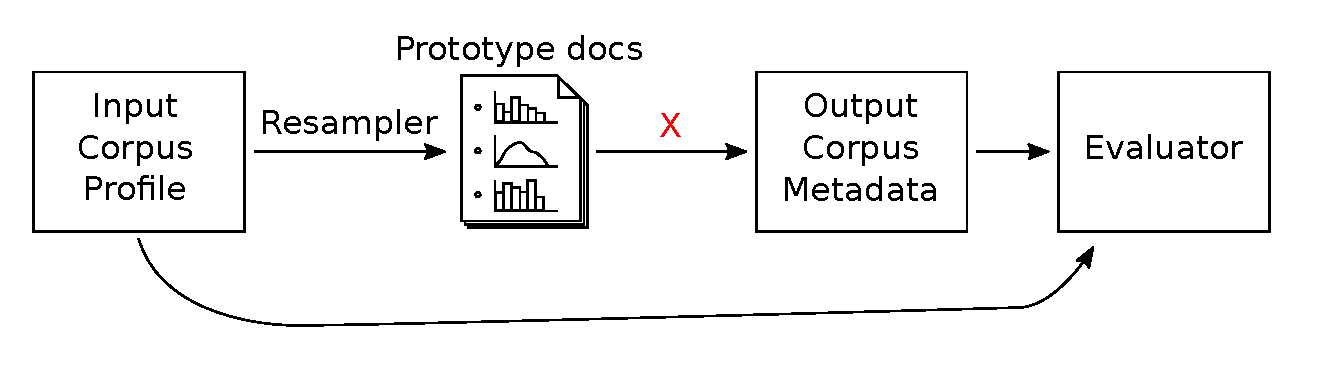
\includegraphics[width=0.9\textwidth]{evaluation/resample-overview}
    \caption{Data flow for evaluation of the sampler.}
    \label{fig:evaluation:resampling:overview}
\end{figure}


The data flow outlined in Figure~\ref{fig:evaluation:resampling:overview} is identical to that used for the final selection, with the omission of a retrieval stage at \textsl{\color{red} x}.  This means the evaluation will be performed under the assumption that the retrieval process is always able to find a suitable document.  The operation performed by the evaluator is essentially a comparison between two distributions, and may be performed using any number of algorithms with the one requirement being that it can practically be executed after each document is retrieved (note that for the purposes of this evaluation, such a requirement is less critical).

Evaluation methods provided in the prototype implementation are:

\begin{itemizeTitle}

    \item[Mean Error] For each dimension, the sum of the deviance from each document to its target value is divided by the number of documents in the collection.  This provides an asymmetric form of the commonly-used Mean Squared Error.
    \item[Distribution Comparison] A commonly used method for comparing empirical distributions, this is computed by taking the differences between the cumulative density of each dimension's data and is thus less sensitive to order than MSE methods.  Typically these methods are able to provide confidence bounds related to statistical significance.
    \item[Linear Modelling] A linear model is constructed and fit with parameters according to the input dimensions.  If this model proves statistically equivalent to the null model, then the residuals are considered uniform.

\end{itemizeTitle}


For the purposes of this evaluation, a distribution comparison method, Log-likelihood, was selected due to its known statistical bounds and wide use in corpus linguistics\footnote{It it worth noting that the log-likelihood statistic is just one of a large number of valid goodness-of-fit tests, the main contender being two-sample Kolmogorov-Smirnov}.  The major disadvantage of using this method, that it is harder to directly relate to the content of each text, is not relevant at this stage of analysis.


Log likelihood comparison methods are already widely used in corpus linguistics for keywording and corpus comparison, and measure significance (using Wilks' theorem\cite{wilks1938large}), rather than effect size (as with many information-theory-based deviance measures such as MI and Jaccard).  This evaluation makes use of such properties in that we desire to know at what point the output distribution is, to a given standard of probability, drawn from the same population as the input.%: as we do not control the size of the input distribution we are unable to control the ultimate power of the test and thus the effect size.

This comparison of the output and input distributions was repeated as documents are re-sampled, the point at which the two cease to be significantly different noted.  This process should establish both RQs:

\begin{enumerate}
    \item Load input corpus;
    \item Repeatedly sample from the input corpus, inserting documents into the output corpus;
    \item After each document, compare the output distribution to the input.
\end{enumerate}


Note that this method treats each metadata dimension of the input corpus as an independent distribution, effectively evaluating the joint distribution of the sample.  This was done to permit comparison where obtaining a sample large enough to provide sufficient statistical power is largely impossible---even in the BNC, there are seldom many documents that share \textsl{all} metadata values.  This has the effect of weakening the test such that the `Conditional' sampler is indistinguishable from the `Marginal' sampler (as mentioned in Section~\ref{sec:rebuilding:method:retrieval:resampling}).



\subsection{Results}

The evaluation here focuses on categorical values with over five members due to the asymptotic nature of the log-likelihood statistic making it unreliable below this number.  As such, the word count was grouped into 17 bins, and the true BNC readability category was used rather than the (continuous) Fleisch reading ease score.  This results in three variables that must converge prior to similarity being determined:

\begin{itemizeTitle}
    \item[Genre]  The genre category, as fit using the classifier heuristic mentioned elsewhere, only using all 70 categories;
    \item[Words]  The word count, binned to form bins with no fewer than five texts in each;
    \item[AudLvl] Audience level, categorised as `high', `med', and `low';
    \item[Mode]   \textbf{S}poken or \textbf{W}ritten.
\end{itemizeTitle}

The word count is binned irregularly due to the low frequency of files with more than 80,000 words listed in the index.  This results in a distribution shown by the histogram in Figure~\ref{fig:evaluation:resampling:bncwordhist}, with the minimum bin frequency being 8.  Other variables were left unmodified.


\begin{figure}[ht]
    \centering
    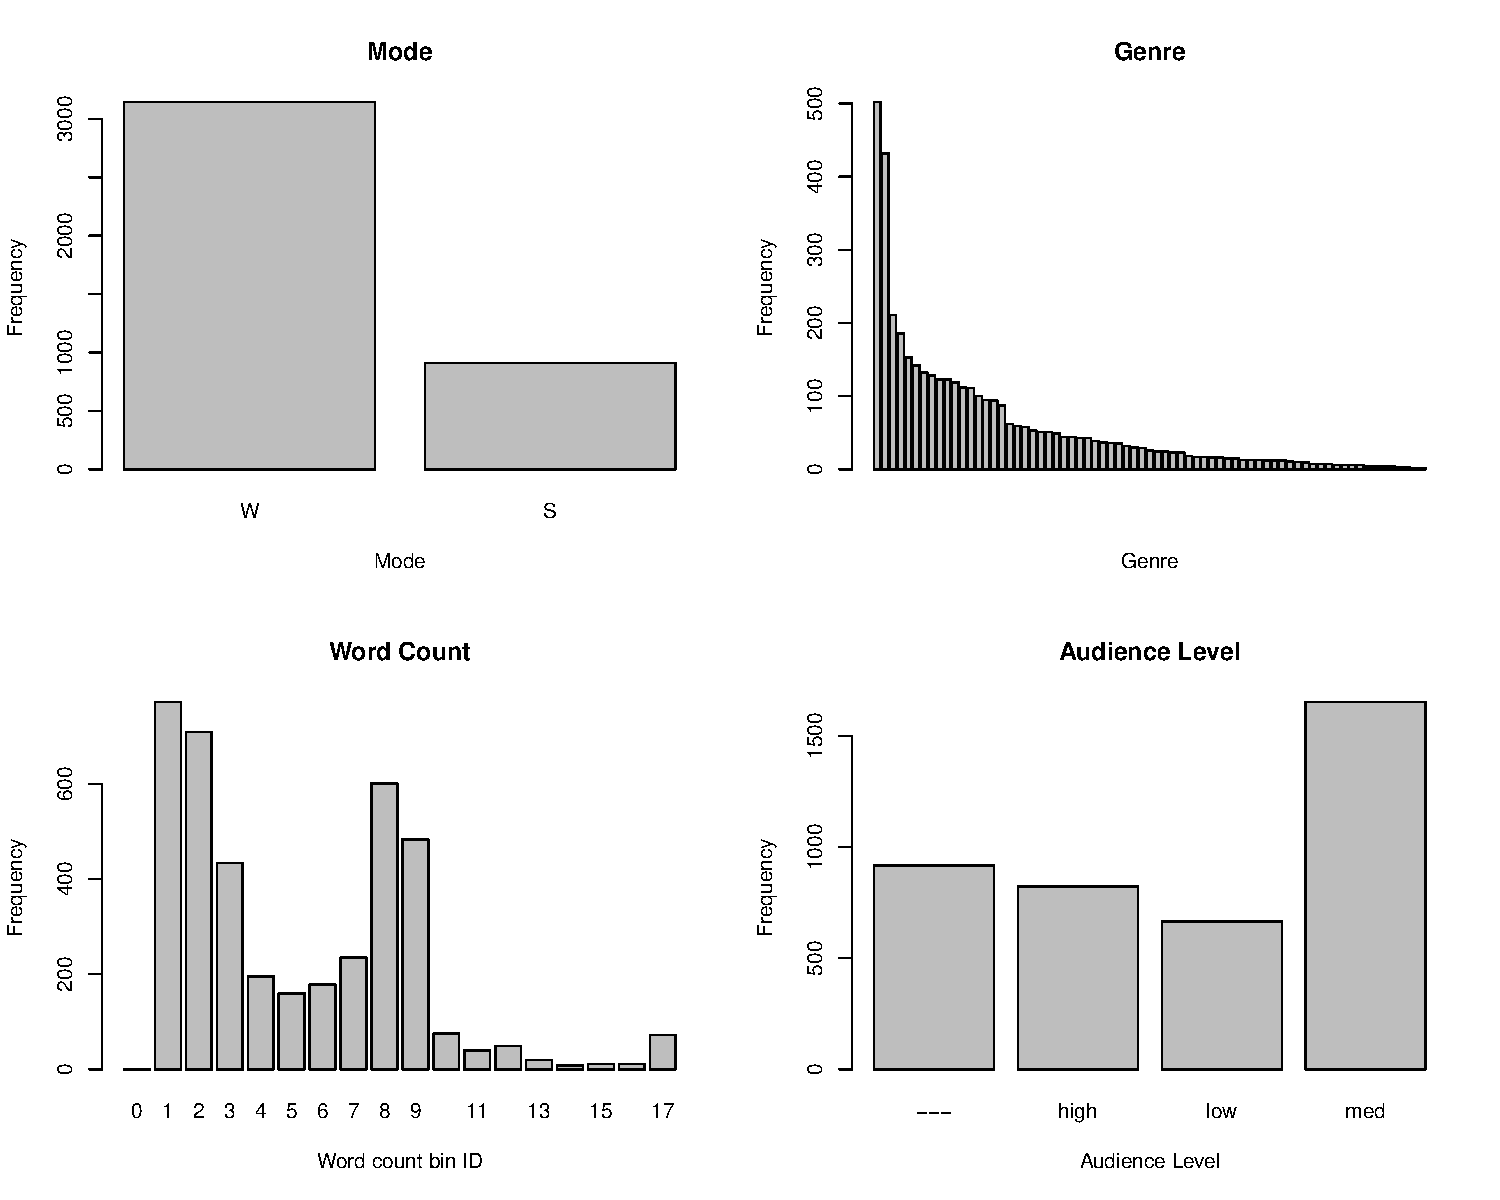
\includegraphics[width=1\textwidth]{evaluation/4waybnchist}
    \caption{Word count distribution from the BNC index (n=4,054, breaks at 5k < 80k, max=428,248)}
    \label{fig:evaluation:resampling:bncwordhist}
\end{figure}


The convergence rate of each of the variables is, as mentioned above, dependent on the information content of the input bins' frequencies (due to the complexity of the sample) and the number of bins with fewer than five members (due to log-likelihood converging slowly to the $\chi^2$ distribution).  Each variable's convergence may thus be appropriately expressed in terms of how long the average bootstrapping process takes to converge upon the distribution to a given confidence value, relative to the size of the input.

A basic description of the bins used for each input metadata item is presented in Table~\ref{table:evaluation:resampling:inputdist}.  Medians and interquartile ranges were used as centrality and deviance measures due to the Zipfian nature of the bin distributions (a feature expected to manifest in most corpora).  The `ID' column gives the `index of dispersion'---a normalised measure of the variability in the distribution's bins computed by dividing the centrality measure (median) by the dispersion measure (Inter-Quartile Range).

% TODO: table with variable, bin count, num<10, stdev, mean, convergeance mean, convergeance confint@95%
\begin{table}[ht]
    \centering

    \begin{tabular}{|l|c|c|c|c|c|}
        \hline
        Metadata & bins & $|n_{bin} < 10|$ & $median(n_{bin})$ & $IQR(n_{bin})$ & ID  \\
        \hline
        Genre & 71  & 16 (22.5\%)   & 26    & 49        & 1.88    \\
        Words & 18  & 2 (11.1\%)    & 117.5 & 359.25    & 3.05    \\
        AudLvl& 4   & 0 (0\%)       & 869   & 317.5     & 0.36    \\
        Mode  & 2   & 0 (0\%)       & 2027  & 1117      & 0.55    \\
        \hline
    \end{tabular}
    \caption{Distributions of metadata dimensions in the input corpus (BNC index)}
    \label{table:evaluation:resampling:inputdist}
\end{table}

The figures in Table~\ref{table:evaluation:resampling:inputdist} represent common cases for real-world corpora:

\begin{itemize}
    \item `Mode' is a simple binary classification with very different group sizes;
    \item `AudLvl' is a simple classification with a relatively `flat' distribution;
    \item `Words' is a bimodally distributed measure with a large amount of variation but also very large numbers in each bin.  This is a good representation of the counts of many linguistic features;
    \item `Genre' is moderately heterogeneous, yet has a distribution with many low-frequency items in it.
\end{itemize}

We may reason from the index of dispersion that convergence will occur faster for `AudLvl' and `Mode' than for `Genre' and `Words' --- the ordering of the other two largely being determined by the conservative estimation of log-likelihood for low-frequency bins.


\begin{figure}[ht]
    % ./analysis/loglik-significance.r
    \centering
    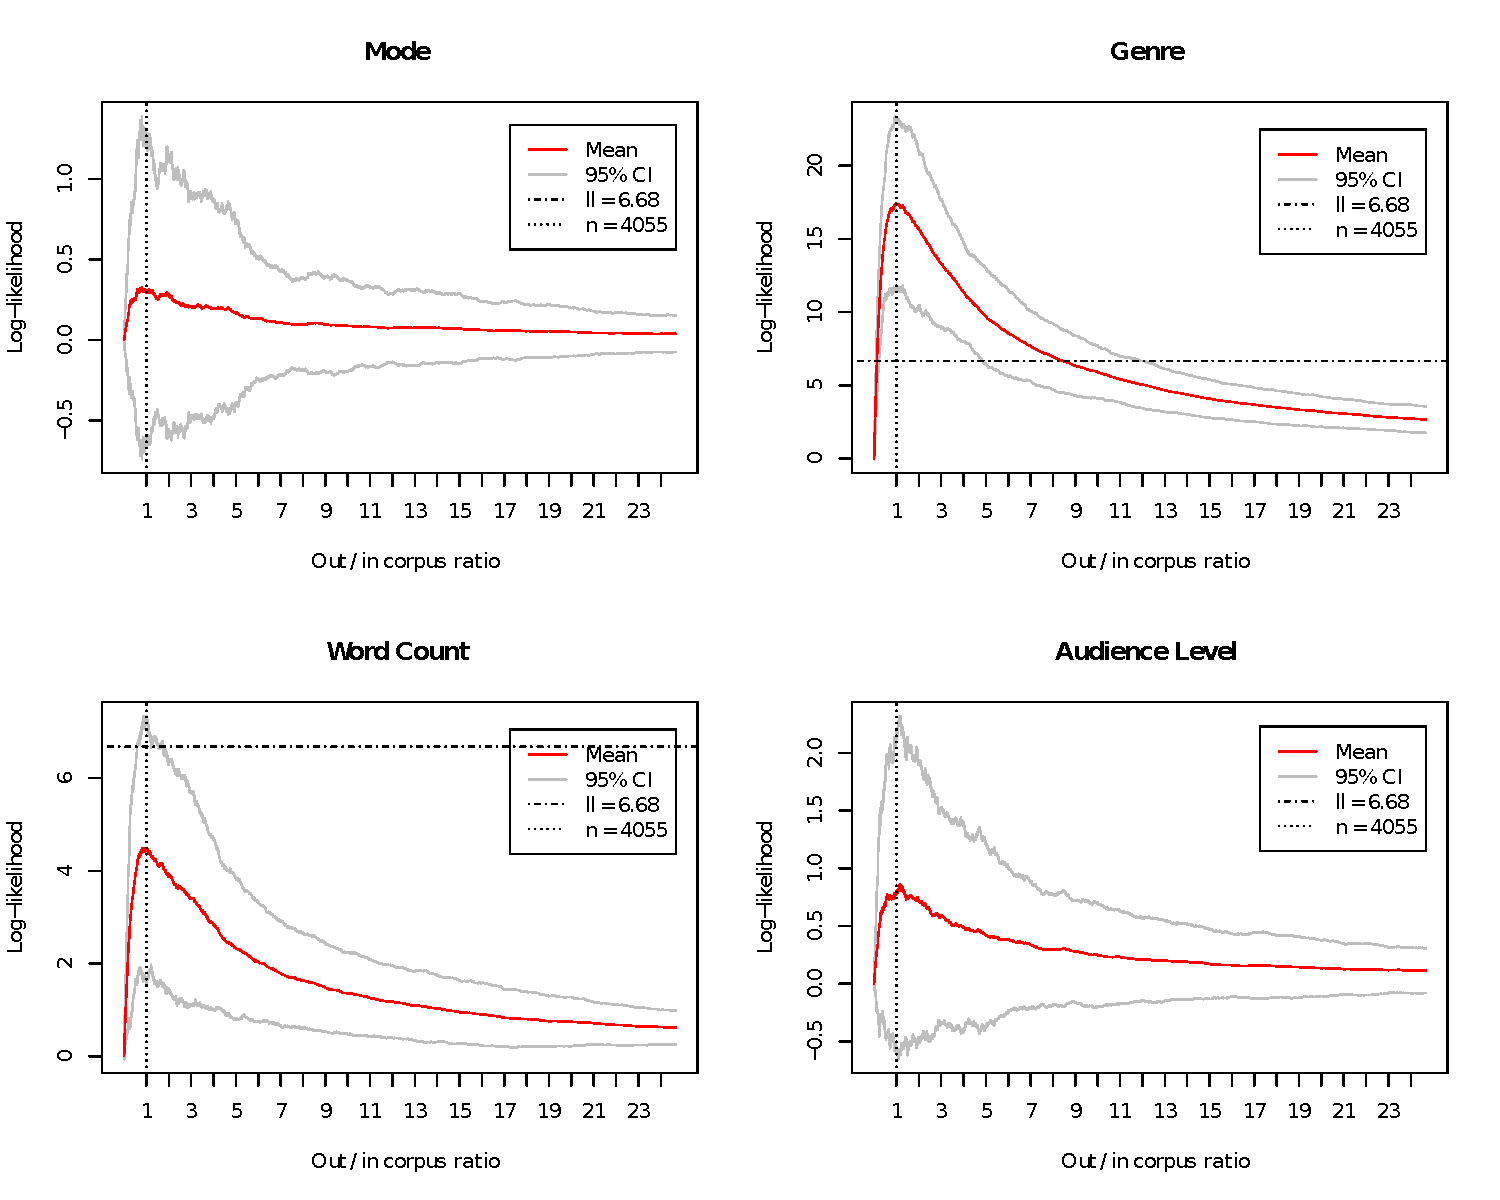
\includegraphics[width=1\textwidth]{evaluation/4wayCI95}
    \caption{Log-likelihood scores and 95\% confidence intervals for each metadata property during resampling (100 repetitions of 100,000 documents)}
    \label{fig:evaluation:resampling:4wayCI95}
\end{figure}


Figure~\ref{fig:evaluation:resampling:4wayCI95} displays the log-likelihood score of the output distribution as it is built.  These graphs clearly illustrate the relative complexity of the input distributions, as well as the downsides of estimating log-likelihood measures for low-frequency results.  After an initial burn-in period, all dimensions gradually converge upon the target distribution.  For any input distribution with low counts, the similarity measure will not be accurate until these lowest bins are filled---marked on the graph roughly as the point where the output distribution is equal in size to the input.%\td{though this is not entirely precise and I think is estimable using binomial}.

The two simpler distributions, `Mode' and `AudLvl', peak at levels well below the 95\% threshold chosen for the log-likelihood statistic.  In the case where the `target' input distribution is defined by profiling an existing corpus, this implies that we could properly build a corpus \textit{smaller} than the input (though unfortunately this is not rigorous without also knowing the relationship of the original input corpus to the population as it is itself generated from that sample).  The relatively confident estimates for these parameters at a 1:1 input:output ratio backs up the rational expectation that large numbers of documents in few bins will be easy to replicate.

A marginally more complex distribution of metadata in the form of the `Words' dimension shows, again, fast convergence, requiring an output distribution roughly twice the output to replicate with 97.5\% confidence.

By far the most complex input data, `Genre', takes much longer to converge, requiring a ratio of roughly 12:1.  This result is largely a function of the low bin frequencies and the large proportion of bins that have values below the threshold at which log-likelihood may be relied upon to provide a moderately-conservative estimate.

The speed of convergence reflects the variability that is permitted in any subsequent retrieval process: fixing the `Mode', for example, will lead to a corpus with known proportions of spoken and written text, but variability otherwise according to the population from which they are sourced.  If a particularly large corpus is available with a desirable sample design, restricting only one dimension merely refines the original sample\footnote{Of course, such a situation is difficult if the corpus from which documents are not tagged with relevant metadata, something unlikely if that dimension was not already in the sample design}.

\paragraph{}

The process of random resampling detailed here is in many ways uninteresting: after all, the experiment detailed above merely selects items based upon existing metadata.  The value in the above technique lies in its mode of use:

\begin{itemize}
    \item The distribution converged upon is arbitrary, and may be defined in the absence of an input corpus (or as a modification thereof).  This allows relaxation of a corpus description's requirements to reduce the necessary oversampling ratio above, or the addition of specific metadata items where the source of documents is particularly easy to sample according to certain properties.
    \item Halting the resampling process at any stage, due to the random selection method used, leads to an unbiased output corpus (though it may well be imprecise).
    % \item After resampling of candidate documents through a process of resampling (which has known bounds of error), the process of retrieving documents can be compared against a gold standard.
    \item When starting with a manually-designed corpus (which has bin sizes only relevant to one another), convergence can only be achieved where the output corpus size is greater than or equal to that of the input corpus.  Aside from fitting issues where bin sizes are small, corpora fit using the same distribution shape should converge at the same size (i.e. \textsl{not} relative to the input corpus size).

\end{itemize}


% TODO: Experiment on convergion point by input n, and/or autocorrelation
% linear models for each, comment on confidence



% ---------









% \til{integrate the below better, it was written standalone.}


The relationship described by the log-likelihood scores of the two corpora describes the confidence one may have in the original, input, corpus: an input corpus with very few documents in each `bin' is less powerful when used to answer questions using data in that bin, and so will require a greater number of documents in the output corpus to achieve confidence at the same effect size.  This is a useful effect, as it ensures that samples are never output that are not in some way large enough to be confident about their distribution, thus enforcing a minimum sample size.  Unfortunately, if this comparison is based on duplication of an existing sample (such as in this case) such an adjustment is non-rigorous as it is based upon the sample parameters, which have an unknown relationship to the population parameters they estimate.  Essentially, whilst this is a heuristic indicating internal validity, it does not ensure external validity.

A notable property of the resampler is that, even if the confidence of the output corpus being `converged' to a given confidence level is very low (i.e.\ the log-likelihood score is above a chosen threshold), the output corpus is unbiased relative to its input due to random selection.  In addition, the convergence of a corpus with a simpler design than the source corpus will occur at a number of documents lower than that of the input corpus, making it possible to resample an existing corpus using a design with \textit{simpler} metadata properties.  In this case, the `simplicity' of the design is defined by the information in the design distribution relative to the information content of the source corpus.  For example, if our experiment did not care about genre, it would be possible to sample texts directly from word count and audience level, producing a corpus with fewer texts yet the same coverage of those two dimensions.
%a mere \td{n} nexts in with a \td{n\%} confidence of representing the input corpus.






% \begin{lstlisting}[language=,caption={Example output showing the recursive resampling process.},label=lst:evaluation:resampling:resampleexample]
% example of running the thing:

% Loading profile...
% [genre] Loading classifier data from memdump: ./resources/list_classifier_dump.dat...
% Loading corpus from /tmp/test.corpus...
% Building sampler for corpus #<Corpus:3:269543840>...
% Using full conditional sampling with Z = 1.645, sd = 30
% Creating (virtual) output corpus...
% Corpus created using 3 dimensions of metadata:
%   - GENRE of type #<Impute::DiscreteDistribution:0x000000025d2710>
%   - Word Total of type #<Impute::SmoothedGaussianDistribution:0x000000025d26c0>
%   - Aud Level of type #<Impute::DiscreteDistribution:0x000000025d2648>
% Selecting random document from #<Corpus:3:269543840>...
%  - dims: 3, docs: 4054
%  - dims: 2, docs: 4 (Word Total == 32528.538691473)
%  - dims: 1, docs: 1 (Aud Level == low)
% => #<Impute::Document:0x0000002123f3b8
%  @dimensions={"Word Total"=>32528.538691473, "Aud Level"=>"low", "GENRE"=>"W_pop_lore"},
%  @id="115f72d0-94cc-4c4d-91d1-6b8cbe18a081",
%  @meta={},
%  @text="">
% \end{lstlisting}







\section{Performance of Retriever}
\label{sec:evaluation:retrieval}
The purpose of the resampling process above is to present well-defined document prototypes to a retrieval stage.  There are many potential sources for document retrieval according to this prototype, including the original input corpus, a separate `super-corpus', or, ideally a separate population (that is itself not a sample).



\subsection{Method}
\label{sec:evaluation:method}

The proof-of-concept evaluated here implements a mechanism similar to that of BootCaT\cite{baroni2004bootcat}, using a search engine to retrieve results based on key n-grams.  This mechanism was selected due to the pertinence of its method to other corpus building efforts---there is no technical limitation imposed by the software tool, and users are free to select any other source of data or mechanism of retrieval.

The similarity of the retrieval system described here to BootCaT, along with the use of concrete prototype documents, allows us to inspect the `measurement error' of using search engines to retrieve data based on key terms.  This evaluation is, therefore, primarily an assessment of that bias and a preliminary assessment of its sources.

% ---

\begin{figure}[ht]
    % ./analysis/loglik-significance.r
    \centering
    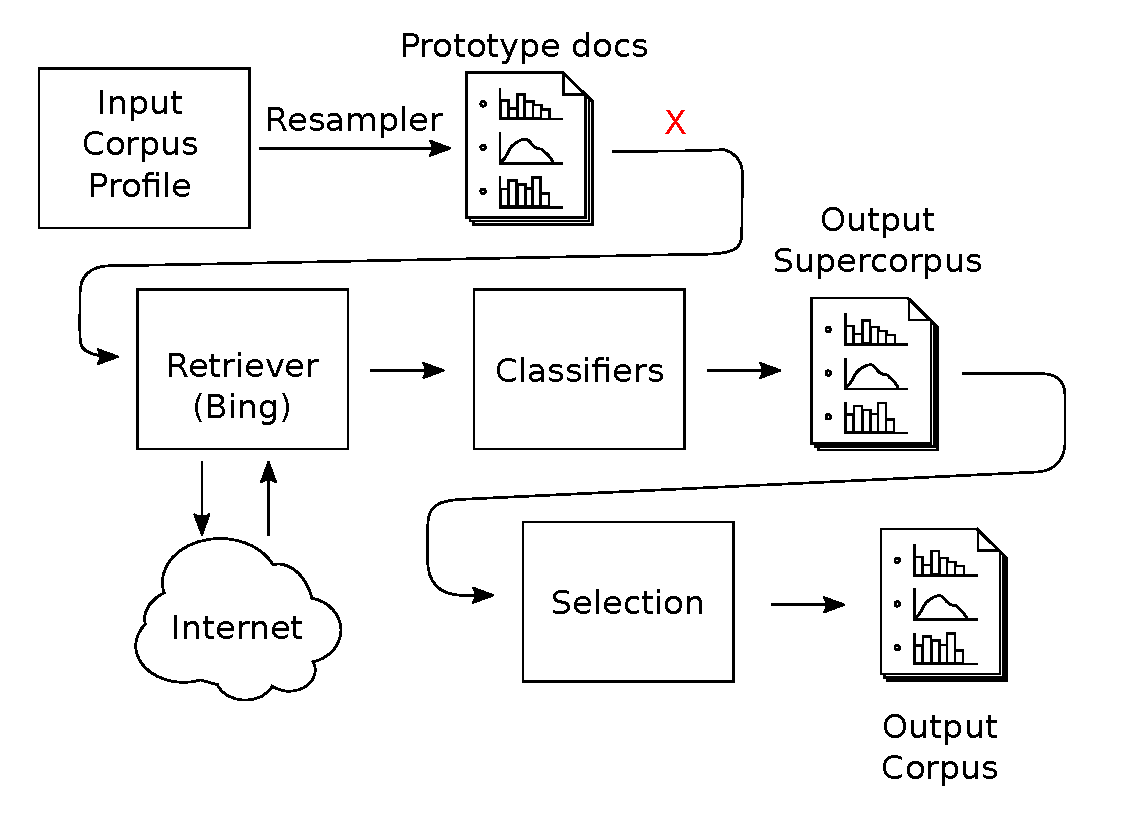
\includegraphics[width=0.9\textwidth]{evaluation/retrieval-overview}
    \caption{An overview of the retrieval mechanism used in the proof-of-concept implementation.}
\label{fig:evaluation:retrieval:outline}
\end{figure}


The retrieval process (as summarised in Figure~\ref{fig:evaluation:retrieval:outline}) is performed iteratively using the components evaluated in the previous sections:

\begin{enumerate}
    \item Sample a prototype document from the corpus profile;
    \item Retrieve candidate links using the Microsoft Bing search engine\footnote{\url{https://datamarket.azure.com/dataset/bing/searchweb}};
    \item Download, remove boilerplate (using JusText\cite{pomikalek2013justext}), and classify each document using heuristics from the corpus profile;
    \item Measure distance in the resulting vector space according to each heuristic's value.
\end{enumerate}

For this data set, both the direct links from Bing and the first level of hyperlinks in each document were downloaded.  Spidering was performed in order to ensure that the sampled area of metadata is a supersample of the desired distribution, as well as to maximise the chances of finding suitable points in other, uncontrolled, dimensions.

Documents with fewer than 100 words were discarded as they were unlikely to be classified accurately.  This could be worked around by selecting 100-word samples from larger texts if necessary.

For this evaluation, the written portions of the BNC were used as the seed corpus.  Keywords used for search were generated using log likelihood scores, and no cutoff was used: instead, the random selection algorithm was weighted by the resulting score.

The spoken and \texttt{W\_Misc} categories were omitted for a number of reasons.  Spoken data was omitted on the conjecture that it is difficult to find online~\footnote{Retrieval of transcriptions may be facilitated by searching for genre-specific features in addition to keywords, and this form of specialism is a potential avenue for improving the accuracy of all genres.}, leading to a predictable gap in the resulting corpus.  \texttt{W\_misc} was omitted due to the need for an accurate classification step, and because keyword-based retrieval requires that said keywords are highly representative of a given genre.  Both of these issues are potentially solvable in future work, yet lie outside the scope of this thesis.


The retriever must, as far as possible, return documents according to \textsl{all} prototype metadata dimensions, that is, it must perform the equivalent to an agglomerative query.  This is a particular challenge for search engines due to their generality.  Since the Bing API lacks tools to filter by any of the three dimensions used in this evaluation, the primary focus was on genre---word count and reading ease were both free to vary.  Language was specified as \texttt{en\_GB}.

% TODO: Write in discussion about how this is challenging but that a hybrid system might work best, say retrieve from scholar if it's a paper.









% This process is deliberately agnostic of any internal variables: the \textsl{content} of the retrieved texts is also affected by the choice of retrieval mechanism, however, this is part of the variance desired in the dataset, and should form part of any motivating research question.

% The problem of when the output corpus is `sufficiently large' may not be solved using this method: whilst the convergeance of the output corpus to the input is known to some degree of certainty, the same cannot be said of the errors in retrieval.  Assuming that each text is entirely accurate to its prototype will yield a corpus showing the same distribution as the input, but this does not mean that the source used is presenting data in an unbiased manner, or that sufficient variation has been captured to generalise about \textsl{that} population.

% It is also possible to select documents that are not a perfect fit to the prototype: indeed, this may be necessary where continuous measures are used to characterise the sampling design.  In this case, the residual variation may be used to determine bias in the selection method by measuring how non-uniform the distribution of these residuals is.  Note, however, that even uniform nonzero residuals represent an overall increase in dispersion compared to the input distribution: it is almost certainly more useful to deliberately apply this to the input distribution by applying a smoothing method prior to resampling than it is to rely on the document retrieval stage (which may apply said dispersion in less predictable ways).

% \til{
% further work:\\
% Though not implemented here, it is possible to use this known error distribution as a correction mechanism for the sampler, deliberately seeking to `shore up' the residuals.  This kind of feedback loop is used in bootstrapping algorithms such as Gibbs and slice sampling, though its application to a procedure based on a fairly hard-to-predict search mechanism (web search engines) presents major engineering challenges.
% }

% % --



% The retrieval method used here (outlined in Chapter~\ref{sec:rebuilding} and Figure~\ref{fig:evaluation:retrieval:outline}) is based on the principle of heuristically seeking documents fitting the prototype, followed by a ranking stage and selection of the highest-ranked document.  This means that it has the potential to output imperfect documents but is maximally unlikely to do so.  It does not adjust for any accumulated error during execution, so has the potential to gradually accumulate errors in one particular direction if `perfectly matched' documents are not available within the parameters given.  This approach is largely taken to prevent the retriever from searching endlessly for a combination of metadata values that simply do not exist in the sources to which it has access: many specific uses of this technique will be able to use far more certain methods for their retrieval stage (up to and including manual selection of documents).








\subsection{Results}
\label{sec:evaluation:results}

In total $72,540$ documents were downloaded after $6,510$ requests to Bing.  After boilerplate removal using JusText\cite{pomikalek2013justext} and discarding of short documents, $55,790$ documents remained in the corpus.


This sample size is $\approx 21$ times the input corpus.  Estimating using graphical methods (as in Section~\ref{sec:evaluation:resampler}, this should be sufficient to provide an appropriately distributed sample of genres.  The worst case is that each Bing search returns very few documents with the desired genre, for example, if each search returns only a single document of interest then this ratio is reduced to $\approx 3n$.



% \subsubsection{Univariate Properties}
Before inspecting the results from the retriever, the limitations of this method should be noted.  Firstly, the ideal retrieval mechanism should target all dimensions of the prototype document provided, in this case Genre, reading ease, and word count).  Bing does not index the latter of these two, leaving them to vary naturally.

This variation interacts with the genre itself, and so it is not possible to generalise from the observations here to the wider web.  The distributions shown in Figures~\ref{fig:evaluation:retrieval:flesh} and~\ref{fig:evaluation:retrieval:words} are, however, indicative of the documents found via Bing when searching for BNC terms.  Upholding the assumption that the written BNC represents general-purpose language use, this is an indication of users' exposure to documents online.%\footnote{This is a distinction drawn strongly amongst WaC, where many efforts attempt to describe the web itself rather than usage thereof.}.

From the point of view of one sampling documents to form a supercorpus, it is desirable that the uncontrolled dimensions are widely and evenly dispersed across the vector space, such that any subsequent rejection sampling is simplified.


\begin{figure}[ht]
    % ./analysis/
    \centering
    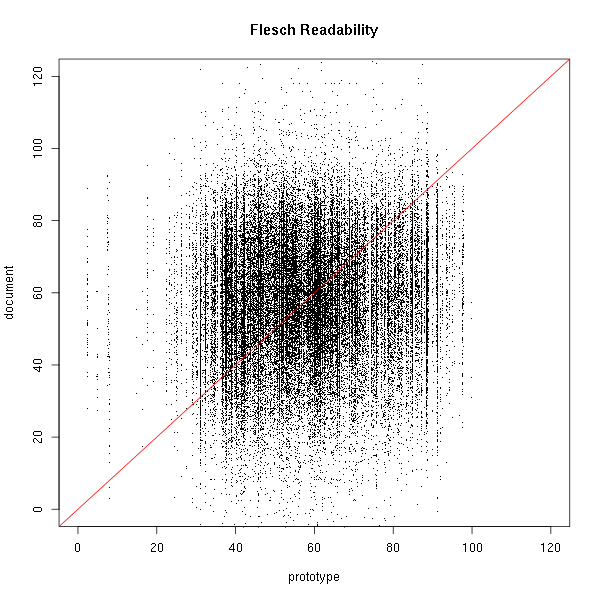
\includegraphics[width=0.8\textwidth]{evaluation/retrieval-flesch}
    \caption{Prototype/document readability scores}
    \label{fig:evaluation:retrieval:flesh}
\end{figure}

\begin{figure}[ht]
    % ./analysis/
    \centering
    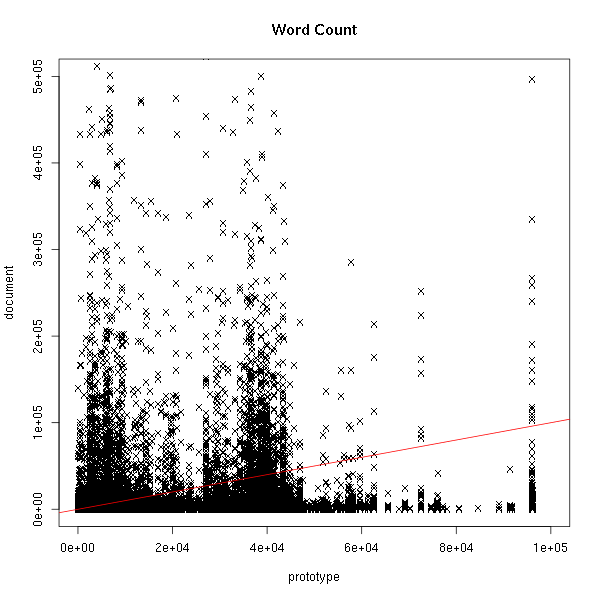
\includegraphics[width=0.8\textwidth]{evaluation/retrieval-words}
    \caption{Prototype/document word counts}
    \label{fig:evaluation:retrieval:words}
\end{figure}

Figure~\ref{fig:evaluation:retrieval:flesh} shows the distribution of reading ease scores across the collected documents, the $y$ axis showing the values as downloaded from the web.  The red line is plotted with a gradient of $0.5$, and shows the ideal zone where documents should lie if retrieved perfectly.


The readability dimension (Figure~\ref{fig:evaluation:retrieval:flesh}) is fairly well dispersed, indicating that there are no documents fundamentally unreachable using the search engine method.  Though this dimension is the simplest, both the prototype and retrieved documents have similar standard deviations ($16.2$ and $17.9$ respectively) and means ($57.5$ and $57.4$ respectively).  There is very little correlation between prototype and retrieved values: with a correlation coefficient of just $0.06$.  Generally, this indicates that most distributions of readability are `covered' online, and the one used in the BNC is easily represented.

\begin{figure}[ht]
    % ./analysis/
    \centering
    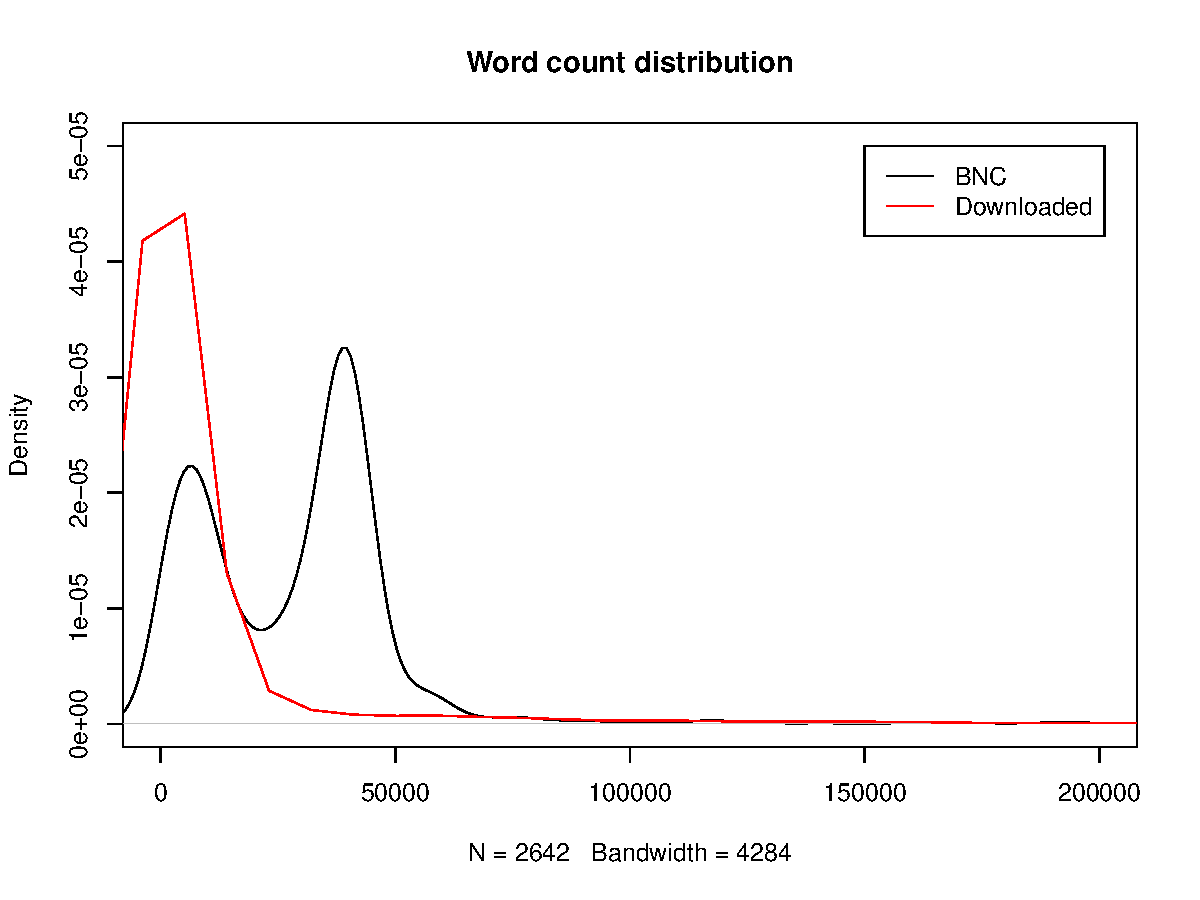
\includegraphics[width=0.8\textwidth]{evaluation/retrieval-words-dist}
    \caption{Distribution of document lengths in the written BNC and downloaded corpora}
    \label{fig:evaluation:retrieval:words-dist}
\end{figure}

Word counts are altogether more complex.  The word count is distributed in the BNC in a far more complex manner (Figure~\ref{fig:evaluation:retrieval:words-dist}), and the method of sampling can be reasonably expected to impact this more than readability.  This shows that the distribution of word counts online (conditioned on genre) is far from that in the BNC: the line of intended fit failing to intersect with longer documents.
% TODO

The distribution plots in Figure~\ref{fig:evaluation:retrieval:words-dist} display the obvious missing portion of the word count target distribution.  This is a clear example of the bias of online documents, which tend to be paginated even where the content is particularly long (a trend that is exacerbated by advertising-based funding models).  The bimodal distribution of the BNC's word counts can be attributed to interactions with `domain'%
%\td{define domain re. lee}\footnote{CHECK LEE's BNC COMMENTS ON DOMAIN}
: with \texttt{W\_world\_affairs} and \texttt{W\_imaginative} forming the bulk of the longer texts.

% \til{
% In the discussion section, mention that this bias can be worked around for most analysis by not sampling whole texts, but that it is an interesting finding that the web can't do long texts.  Perhaps refer to this in the keyword bit later.
% }



\begin{table}[ht]
    \centering

    \begin{tabular}{|r|l|r|r|r|r|}
        \hline
        & Genre & Prototype & Downloaded & TP & TPR (\%) \\ 
        \hline
        1 & W\_ac\_humanities\_arts & 2180 & 1089 & 181 & 8.30 \\ 
        2 & W\_ac\_medicine & 987 & 1162 & 415 & 42.05 \\ 
        3 & W\_ac\_nat\_science & 684 & 1258 & 160 & 23.39 \\ 
        4 & W\_ac\_polit\_law\_edu & 4424 & 1467 & 590 & 13.34 \\ 
        5 & W\_ac\_soc\_science & 3112 & 1074 & 290 & 9.32 \\ 
        6 & W\_ac\_tech\_engin & 466 & 1267 & 129 & 27.68 \\ 
        7 & W\_admin & 195 & 1038 & 23 & 11.79 \\ 
        8 & W\_advert & 856 & 4501 & 273 & 31.89 \\ 
        9 & W\_biography & 2979 & 1736 & 221 & 7.42 \\ 
        10 & W\_commerce & 2952 & 2058 & 464 & 15.72 \\ 
        11 & W\_email &  46 & 882 & 3 & 6.52 \\ 
        12 & W\_essay\_school &   1 & 871 & 0 & 0 \\ 
        13 & W\_essay\_univ & 246 &  23 & 0 & 0 \\ 
        14 & W\_fict\_poetry & 815 & 460 & 42 & 5.15 \\ 
        15 & W\_fict\_prose & 10487 & 1844 & 888 & 8.47 \\ 
        16 & W\_hansard & 161 & 114 & 39 & 24.22 \\ 
        17 & W\_institut\_doc & 572 & 1952 & 131 & 22.90 \\ 
        18 & W\_instructional & 111 & 941 & 54 & 48.65 \\ 
        19 & W\_letters\_personal & 124 & 611 & 9 & 7.26 \\ 
        20 & W\_letters\_prof & 227 & 396 & 9 & 3.96 \\ 
        21 & W\_newsp\_brdsht\_nat\_arts & 764 & 3470 & 147 & 19.24 \\ 
        22 & W\_newsp\_brdsht\_nat\_commerce & 792 & 484 & 100 & 12.63 \\ 
        23 & W\_newsp\_brdsht\_nat\_editorial & 212 & 909 & 23 & 10.85 \\ 
        24 & W\_newsp\_brdsht\_nat\_misc & 1544 & 896 & 45 & 2.91 \\ 
        25 & W\_newsp\_brdsht\_nat\_report & 854 & 925 & 73 & 8.55 \\ 
        26 & W\_newsp\_brdsht\_nat\_science & 235 & 284 & 6 & 2.55 \\ 
        27 & W\_newsp\_brdsht\_nat\_social & 881 & 259 & 6 & 0.68 \\ 
        28 & W\_newsp\_brdsht\_nat\_sports & 639 & 503 & 97 & 15.18 \\ 
        29 & W\_newsp\_other\_arts & 216 & 1345 & 49 & 22.69 \\ 
        30 & W\_newsp\_other\_commerce &  91 & 466 & 18 & 19.78 \\ 
        31 & W\_newsp\_other\_report & 756 & 933 & 52 & 6.88 \\ 
        32 & W\_newsp\_other\_science & 327 & 196 & 3 & 0.92 \\ 
        33 & W\_newsp\_other\_social & 904 & 705 & 41 & 4.54 \\ 
        34 & W\_newsp\_other\_sports &  26 & 540 & 4 & 15.38 \\ 
        35 & W\_newsp\_tabloid &  45 & 482 & 2 & 4.44 \\ 
        36 & W\_news\_script & 479 & 121 & 3 & 0.63 \\ 
        37 & W\_non\_ac\_humanities\_arts & 1610 & 1665 & 193 & 11.99 \\ 
        38 & W\_non\_ac\_medicine & 384 & 1605 & 142 & 36.98 \\ 
        39 & W\_non\_ac\_nat\_science & 1438 & 1534 & 258 & 17.94 \\ 
        40 & W\_non\_ac\_polit\_law\_edu & 2891 & 1428 & 463 & 16.02 \\ 
        41 & W\_non\_ac\_soc\_science & 2210 & 1516 & 134 & 6.06 \\ 
        42 & W\_non\_ac\_tech\_engin & 2578 & 807 & 513 & 19.90 \\ 
        43 & W\_pop\_lore & 3371 & 6918 & 662 & 19.64 \\ 
        44 & W\_religion & 838 & 1942 & 400 & 47.73 \\ 
        \hline
    \end{tabular}


    \caption{Document counts by genre for prototypes and downloaded documents.}
    \label{table:evaluation:retrieval:words-dist}
\end{table}

\FloatBarrier{}

\begin{figure}[ht]
    % ./analysis/
    \centering
    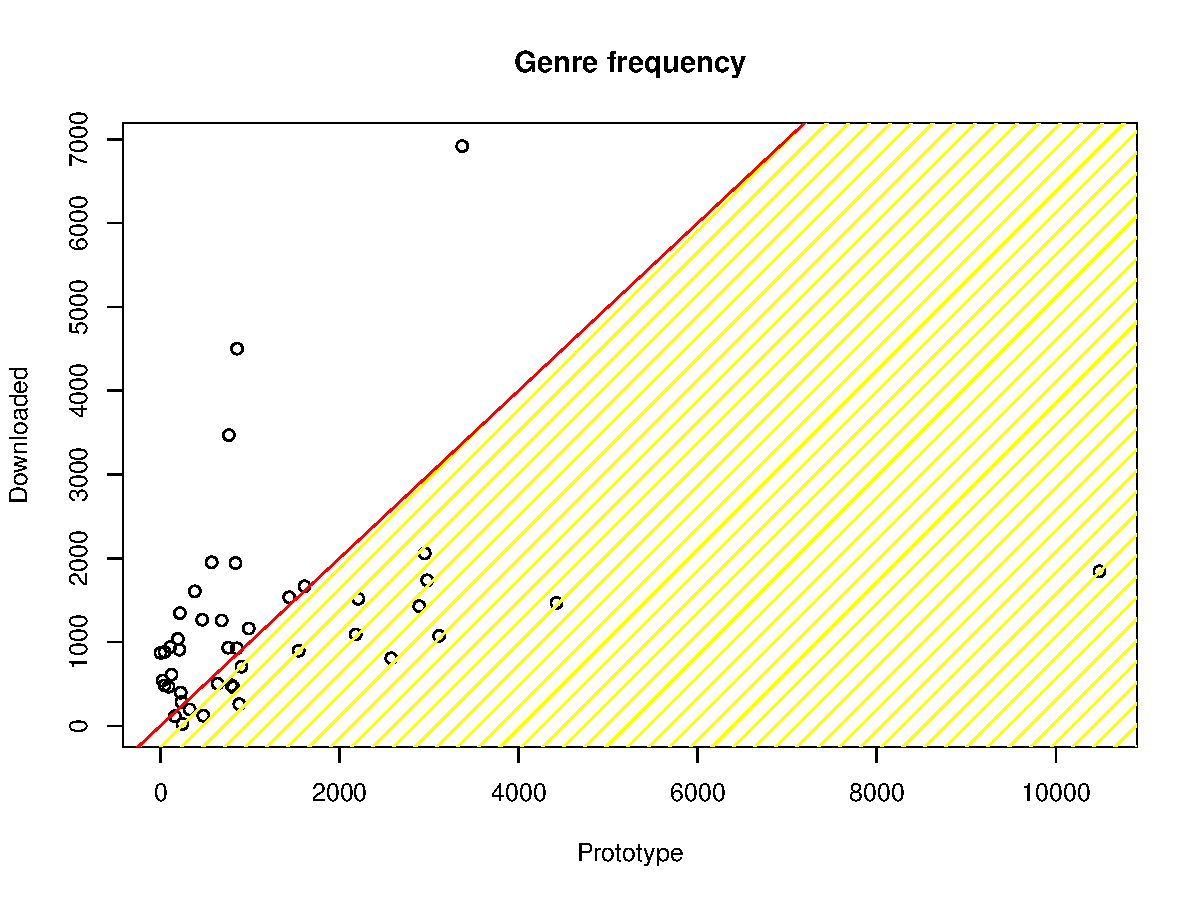
\includegraphics[width=0.8\textwidth]{evaluation/retrieval-genres-corr}
    \caption{Prototype genres frequencies and resulting downloaded document frequencies.  Shaded area indicates `over-downloaded' categories.}
    \label{fig:evaluation:retrieval:genres-corr}
\end{figure}


\begin{figure}[ht]
    % ./analysis/
    \centering
    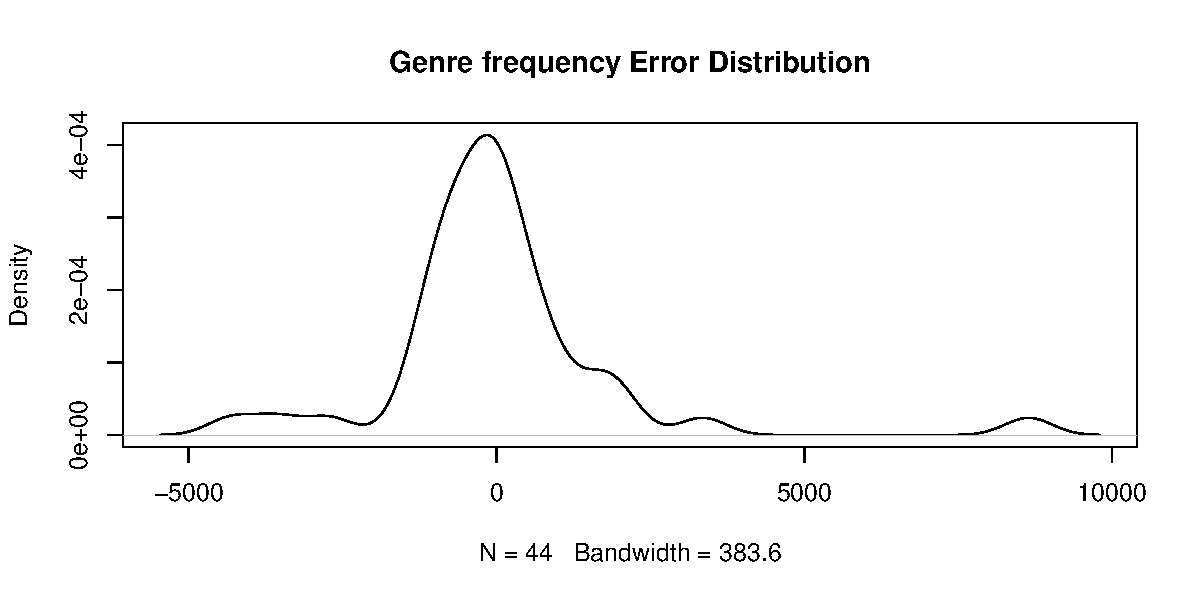
\includegraphics[width=0.8\textwidth]{evaluation/retrieval-genres-diffdist}
    \caption{The distribution of differences in genre frequency between prototype and downloaded documents.}
    \label{fig:evaluation:retrieval:genres-diffdist}
\end{figure}


Genre was the only parameter explicitly controlled-for by the search engine retrieval method.  Precise counts for each of the prototype and retrieved genres are provided in Table~\ref{table:evaluation:retrieval:words-dist}.  

Figure~\ref{fig:evaluation:retrieval:genres-corr} shows the prototype vs.\ downloaded genre frequencies.  Those genres above the line are under-represented in the downloaded documents, relative to the prototype documents\footnote{This measure is distinct from precision/recall in that it does not care which individual documents account for the frequencies, only that the search has retrieved appropriate proportions of each}.
When selecting a full corpus using the search engine lookup method, differences between the prototype and downloaded document classes should be minimal---when selecting a supercorpus, care must be taken to ensure that items in the top-left of the plot have sufficient frequencies for the intended purpose.
% In the ideal casejust $19$ of the $44$ categories have been "over-sampled".

Evidence for the `directedness' of genre-based retrieval using n-grams is given by the dispersion of data around the red line.  Rank correlation between prototype and retrieved documents is $0.45$, and a Mann-Whitney test is not significant ($U = 786.5; p \approx 0.13 > 0.05$), indicating that errors in retrieval are loosely centred around the prototype's frequencies.  This is reinforced by inspecting the density plot for differences between category frequencies, shown in Figure~\ref{fig:evaluation:retrieval:genres-diffdist}.
%This is evidence that retrieval using search terms produces documents similar to those searched for.

% --

Treating the searching process as a classifier allows us to examine the expectation of retrieving a genre successfully.  $7,355$ documents were returned with the desired genre, leading to a true positive rate of $13.2\%$.  This implies retrieval results close to the worst case of one relevant document per search, and explains the low correlation between predicted and resultant class types.  Note that the number of useful documents is above this thanks to re-examination of those previously returned.

Per-class retrieval rates are displayed in the right-most column of Table~\ref{table:evaluation:retrieval:words-dist}.  There is correlation between the size of a genre and its true positive rate ($\rho = 0.29$)%
% Spearman: rho = 0.59
% not sure what this is: ($\rho = 0.84$)
, and inspection of the table indicates that performance is highly variable.  Particularly low retrieval rates (below 5\%) were reported for ten categories.  Many of these are very `general', defined by their context rather than topic: such topics both resist keyword-based retrieval using search engines, and make classification itself difficult once retrieved.  The notable exceptions are the \texttt{\_science} and \texttt{\_social} news categories, retrieval rates of which are likely to be affected by the anachronistic nature of the keyword source (the BNC).  Notably, though retrieval rates were low for these categories, documents were available in all cases, they were simply not the result of that particular search iteration.
% better predicted by the `linguistic specificity' of a given category (with religion, medicine and tech leading the recall rate statistics).

Though it is not possible to separate classifier error from retrieval error without construction of a gold standard corpus (something that lies beyond the scope of this work), earlier evaluations of the classifier used (Section~\ref{sec:evaluation:heuristics:genre}) show that classifier error is not strongly biased.  This allows us to conclude that evidence of significant bias in the resultant data is largely a product of the searching process, rather than document classification.


% -- 



\begin{table}[htb]
    \centering
    \begin{tabular}{|lrrr||lrrr|}
        \hline
        \multicolumn{4}{|c||}{{\bf Over-sampled}}                       & \multicolumn{4}{c|}{{\bf Under-sampled}}                         \\ 
        {\bf term} & {\bf original} & {\bf retrieved} & {\bf loglik} & {\bf term}    & {\bf original} & {\bf retrieved} & {\bf loglik} \\ \hline
        p          & 29217          & 8839489         & 1977900.5    & she'd         & 7338           & 4050            & -17407.3     \\
        s          & 17778          & 1903037         & 357245.2     & darlington    & 5559           & 1521            & -16657.0     \\
        she        & 290860         & 916731          & 136365.1     & ec            & 6091           & 5531            & -11220.7     \\
        gt         & 111            & 535127          & 134335.1     & solicitors    & 2135           & 1086            & -5237.0      \\
        com        & 172            & 465891          & 116044.3     & swindon       & 2182           & 1409            & -4825.7      \\
        www        & 2              & 448772          & 113981.6     & kinnock       & 1375           & 264             & -4466.7      \\
        amp        & 668            & 432633          & 102780.7     & theda         & 838            & 32              & -3297.3      \\
        lt         & 792            & 425436          & 99921.8      & nizan         & 756            & 6               & -3146.1      \\
        had        & 359670         & 1439973         & 94877.1      & cnaa          & 742            & 1               & -3140.1      \\
        h          & 8094           & 555374          & 90772.7      & guil          & 755            & 43              & -2886.5      \\
        t          & 9078           & 557616          & 87217.1      & maastricht    & 1165           & 593             & -2856.9      \\
        her        & 277189         & 1070672         & 80897.8      & oesophageal   & 957            & 279             & -2820.0      \\
        2015       & 25             & 293434          & 74145.0      & lexical       & 1106           & 514             & -2809.1      \\
        2014       & 16             & 254997          & 64517.4      & robyn         & 1200           & 707             & -2767.5      \\
        he         & 523177         & 2629585         & 59109.8      & lamont        & 1184           & 708             & -2712.6      \\
        was        & 722425         & 3866921         & 58399.0      & risc          & 1013           & 416             & -2689.4      \\
        cent       & 34353          & 44410           & 49457.4      & knitting      & 1509           & 1463            & -2668.9      \\
        the        & 5021789        & 33346038        & 47673.9      & athelstan     & 1060           & 516             & -2645.3      \\
        be         & 524709         & 2771036         & 45819.9      & privatisation & 1104           & 665             & -2521.1      \\
        it         & 727487         & 4058706         & 45306.4      & leapor        & 626            & 18              & -2502.2      \\ \hline
    \end{tabular}

    \caption{The 20 most over- and under-represented terms relative to the BNC.}
    \label{table:evaluation:retrieval:keywords}

\end{table}





Finally, keywords were computed relative to the original input corpus using log likelihood.  These offer insight into the specific biases of the data source and a handle on qualitative differences between sampling processes.  

% This is a comparison of the supercorpus against the input used to generate it.
% Should a 'fake' BNC be generated by rejection sampling the supercorpus too?  The comparison would arguably be fairer.


The top 200 keywords\footnote{I recognise that nspection of the top $n$ keywords is not a hugely sound methodology, but it should prove indicative for these purposes} were inspected for the whole supercorpus relative to the seed corpus. Overrepresented tokens were scored separately to under-represented ones in accordance with Baron et.\ al.\cite{baron2009word}, and the lists were free-coded for prominent themes.  The 20 most over- and under-represented terms are displayed in Table~\ref{table:evaluation:retrieval:keywords}.  The full lists are included in Appendix~\ref{sec:appx:keywords}.

Overrepresented terms may be grouped into a number of categories.  The first of these is technical terms: those that are side-effects of the tokeniser or otherwise are related specifically to the web.  This includes features such as protocols (\textsl{HTTP}), and features of URLs (\textsl{co}, \textsl{org}), as well as terms such as \textsl{email} and \textsl{posted} which have simply become more prevalent since the BNC was produced.  It's difficult to say whether or not a more recent seed corpus would eliminate most of these from the keyword list.



Temporal features dominate the rest of the list, with many terms related to date or proper nouns (\textsl{Obama}, \textsl{Nike}).  Dates feature prominently: \textsl{2001}-\textsl{2012} are all mentioned, along with \textsl{1991} and \textsl{1988}.  Genetics is also mentioned (\textsl{gene}, \textsl{mutation}), along with education (\textsl{university}, \textsl{pupils}) and government (\textsl{government}, \textsl{council}).

The remaining terms are pronouns or function words.  These, along with the large number of quantities and references to time/date imply consistency with other WaC datasets, that is, an overrepresentation of news online\cite{sridharan2012modeling}.

This central theme is interesting to contrast against the BNC, which contains a large quantity of news material already, indicating that news genres are even more prevalent online, or that news media (or perhaps just online news) has become more extreme (that is, less similar to other written genres) than the bulk of the BNC data.

Features that are significantly under-represented predominantly fall into the category of proper nouns, and these are mostly political and from the UK (\textsl{Kinnock}, \textsl{Gummer}, \textsl{Heseltine}).  Since the search engine was instructed to search the `GB' marketplace, many of these are most likely explained by temporal effects---the prevalence of these keywords also points at the strength of news within the BNC, along with places and organisations that featured in the news at the time (\textsl{TUC}, \textsl{Maastricht}, \textsl{DTI}).

There is also a strong theme of legal terms (\textsl{offeror}, \textsl{solicitor}, \textsl{arbitrage}), which points at a clear under-representation of legal documents returned by search engines.  This is likely a technical limitation of the retriever, which avoids files in PDF format.

Some technical terms are also presented in the keyword list due to the speed of progress in that field: \textsl{80486} and \textsl{microcomputer} both showing their age.

Finally, there are a number of gastric terms (\textsl{oesophegeal}, \textsl{pylori}, \textsl{duodenal}), which point to a very specific set of documents missing in the returned data.  These terms are from an academic context that, like legal documents, is under-represented for technical reasons, however, it is also likely that the specificity of this category indicates an over-representation within the BNC to some degree.

The relative obscurity of the under-represented terms and the predictable, largely temporal, nature of the over-represented ones is particularly encouraging, indicating that the web is a suitable source for many general-purpose (or current-affairs-focused) applications.


% TODO: Comparison of keywords from data (should be no sig. differences!)

% TODO: possibly also generate a false BNC from the supercorpus and analyse its keywords to see the differences.













\section{Discussion}
\label{sec:evaluation:discussion}


The quantitative data presented above are of limited utility to others, since the degree to which they describe the subject's life (rather than some general linguistic trend) is unknown.  Without further sampling, or detailed linguistic auxiliary data, we cannot begin to generalise from the above in a useful manner.

This does not mean, however, that we cannot reason rationally about how transferrable those results are---it is more unlikely that a member of the general population is a software developer than it is that they watch TV, or listen to BBC Radio 4 in the mornings.

Moreover, since the purpose of the study is to assess the viability of methods, these may be seen as significantly more transferrable than the data they have collected (this distinction is blurred by the inclusion of a human interest model, however.)




% ---------------------------------------------------------------------------
\subsection{Types of data}
The form each corpus takes is rather variable due to the different sampling methods used.  For some sources, e.g.\ books, the personal corpus is likely to contain more partial samples (as books are seldom read in entirety within one `linguistic event').  Those sources that are read piecemeal are also likely to occur multiple times, something that would not be tolerated in conventional corpus designs.
% ---------------------------------------------------------------------------




\subsection{Method}
The process of gathering data itself was optimised for low intrusiveness, and largely proved practical to pursue medium-long term.

Maintenance of the live notebook was the major interruption in everyday language use, and this was gradually optimised to a shorthand format that demanded less time in the field, yet more annotation to extract data.  Where the subject is someone other than the analyst, the format of journals would need to be solidified ahead of time to ensure all properties are identifiable.

On reflection, the mnemonic effects of the notebook were most useful in operationalising the data---the narrative they created placed all other data items in context, and the detailed notes in the nightly journal contribute to an episodic memory that aided the coding process.  Again, this process of reflection is unlikely to be made available to an analyst without explicit insertion of an interview phase where the two may meet to resolve possible misconceptions.

The nightly journal, whilst useful during the study as a place to write down easily-forgotten details of language events, was less useful than anticipated during analysis.  In reality, the richness of the narrative one quickly notes down of a night proved to be difficult to operationalise, meaning that it was largely of use only as auxiliary data to augment the live notebook's event-by-event format.

Some sources of data proved significantly easier to normalise into a workable format than did others.
%(The suitability of each will depend heavily on the form of data one is aiming for when deciding to use similar methods, however).

SQUID logs proved particularly difficult to process largely due to technical reasons, as extensive whitelists and multiple manual inspection phases were necessary to disregard advertising and AJAX requests.  A possible solution to this would be to rely on sampling of web data closer to where it is consumed, for example through the use of a browser plugin.

Initial plans were to use Voice Activity Detection (or full automated transcription) to estimate word counts from verbatim audio recordings.  In practice the diversity of unwanted noise effects (background noise, positioning of microphone, overheard conversations) rendered this practically impossible.  Even rudimentary VAD algorithms work with frequency detection strategies, and many were liable to detect things such as music as continuous speech.  %\td{say more on this}



% ---
Of particular interest to the methodology is the inclusion of a human interest model in the processing stages.  Without this model, the data is changed to massively overestimate the word counts of many data sources (some more than others), and it is the opinion of the subject that the model improves the plausibility of data.  Generalising the method requires generalising this model or narrowing down the number of sources it must cover, either by using more selective data gathering methods or by restricting the scope of the sample.

Each of the data sources mentioned is burdened with its own empirical concerns that must be considered when designing a human interest model, and the general solutions for many of these may be particularly complex.  For example, models for websites using large graphical elements as well as text must take into account Gestalt principles as well as models for humans as they read text, and the particular interests of the subject.

One way this problem may be solved is through detailed elucidation of particular features and interests via a questionnaire or laboratory tasks in addition to the data gathering methods described here.  Clearly, though, relating these to a usefully-complex model of human interest will demand further research.




One of the larger challenges in gathering data from so many sources (and in so many forms) is the amount of work needed to operationalise it.  This was done both manually (in the case of complex data such as photographs and notebook entries) and automatically (for the majority of sources).  Often, some degree of manual correction or annotation was necessary even where automated processing was used.  These processing tools were bespoke, and would need to be generalised if the method is to become viable for use gathering further samples.  The tooling used is summarised in Appendix~\ref{tex/appendices/postprocessing}.



% ---
A number of questions were raised during the sampling period surrounding the limits of data that should be captured.  The solutions used were taken from the subject's own judgement of what constituted language `use' (since this case study is predicated upon recording that opinion), however, further work would be needed to establish answers to these in the general case, and other researchers may be guided by more principles linguistic theory.


The attention models used to narrow down input have already been mentioned, however, they apply at a very specific level---often, shorter texts such as signs, brands and labels would have particularly familiar or conventional text placements, styles, and shapes (some media, such as road signs, deliberately accentuate these features to aid recognition).  It is unclear at what point a text is `read' rather than just recognised in the periphery of one's vision.  The solution used in this study was one of internal vocalisation---if the text was recognised sufficient to repeat/act upon it mentally, it was classed as read.  This means it is often possible to say that a text source had just a few words read, when in fact a number of boilerplate features were skipped over because of their position and style.


An extension of this problem is one of re-reading texts that are being written.  The degree to which this occurs is likely extremely variable by person and task, however, it proves to be a particularly complex form of the above problem and is particularly hard to measure (or even subjectively assess).  In this case study no attempt was made to compensate for this effect.  Detailed study using some kind of attention measuring system (for example, eye tracking) may allow for deliberately using attention coefficients greater than 1 (for word counts) or deliberate repetition of data in the final corpus.


The suitability of the attention system used in this case study is also debatable.  The current method of using a coefficient works only for estimating word counts, and does not favour certain regions of the final data over others.  Additionally, it conflates two effects---that of reading only a small proportion of the source text, and that of paying little attention to the text (you may also consider using a second text at the same time a third form of inattention).  Annotation of simultaneous events was fairly simple in the notebooks, however, estimation of the distribution of one's attention was done only at a low resolution (the codes used practically equate to ratios of 80/20, 50/50, 20/80, 100 with only a few exceptions).





Since the aim of this study was to assess genre proportions, significant amounts of effort were saved by not converting all sources into verbatim text.  This is largely an issue of post-processing, as many methods were digital and thus yielded verbatim text with ease and those that do not have well established transcription procedures.  Of particular note is the importance of being able to apply a regional attention model to extract (or weight) the most read portions of a text, something that (as noted above) was not attempted here due to a focus on proportions and word counts.






\subsection{Sampling Period \& Validity}
It seems clear both from personal reflection and examination of the data, which strongly favours certain work-related activities over others, that a two-week sampling period is hardly enough to represent even an individual's language use.

There are a number of obvious reasons for this, particularly egregious examples being:

\begin{itemize}
    \item Some language sources are usually read slowly, such as books read at bedtime.  A sampling period that covers an individual's various literary interests would have to be very long indeed.
    \item Life is strongly periodic, and though attempts were made to cover the weekly cycle of work and weekend, many events occur annually (either due to seasons or social convention).  There are no Christmas songs in my corpus.
    \item Many more obscure items were represented only once in the corpus (such as advertising on vehicles or documentation on things such as legal forms).  These features may not be periodic but they are temporally rare.
    \item A person's behaviour is likely to be `chunky', following one pattern for a time and then deviating suddenly (for example, during holidays or upon a job change).  Significant effort would have to be given to careful description of duration and circumstance in order to make confident generalisation from the data captured using this method.
\end{itemize}

It is my opinion that this method is up against two major challenges which must be balanced in order to achieve some degree of scientific validity.  The former, and most addressable, of these is the difficulty of sampling in-the-field.  The more obtrusive a method, the higher quality data is going to be, however, the shorter any practical sampling period is likely to be.  The latter, as already discussed, is the problem of generalising between people in order to create a corpus of inter-person language use that retains the same details discussed here.

Given the relative paucity of metadata within many general-purpose corpora and the periodic/temporal complexity of life, it seems reasonable to suggest that an ideal mix would be better formed from long-term (multi-year) samples using low-resolution sampling techniques.  This may entail, for example, discarding the on-line journals and manual photography in favour of automated life-log photography and a nightly journal only.

Following sufficient repetition of short-duration studies, it would be possible to be more confident in the results of longer-term, lower-resolution samples, as the areas with less uncertainty may be attended to less intrusively.







\subsection{Data and Comparisons}
As mentioned in the quantitative section above, there are some large differences between the corpus gathered here and the BNC (here used as an example general-purpose corpus that purports to cover the subject).  It is clear that a number of these are down to individual variation (the technical and musical genre bias), however, other disparities are of an altogether more ambiguous status.

The overall word count of the BNC, and other similar corpora, is called into question by the size of this corpus.  In two weeks, a single person used almost a million words whilst focusing heavily on just a few subjects and roles.  Given the sheer number of people within the British population, their demographic variability, and the dubious extent to which even these two weeks represents our subject's use of language accurately, it seems preposterous to suggest that a mere 100 million (or even billion) words would sufficiently represent language use for almost any purpose.


As previously discussed, the different selection of genres indicates that the BNC's selection of materials is an imperfect superset of the subject's use of language.  It is reassuring that many of the genres absent from the BNC are minor ephemera (signs, tax discs etc.), however, there is a significant underrepresentation of others (mainly technical and broadcast media).  This underrepresentation is partially due to the subject's demographics, something that we would expect to skew the relative proportions of the corpus, and partially due to the age of the BNC, something that is particularly undesirable.



% \til{probably some more...  What is the ratio of variance between a population and the individual, over a given time period?}









\subsection{Validity}
The design of this experiment is subject to a number of challenges to validity.

Perhaps the most severe of these is the extremely personal nature of the corpus itself, which renders verification of the data all but impossible except through elicitation and subjective judgement.  This is to some degree a property of all case studies, especially those seeking to experiment with methodology.

A strong case has been made in many fields (and by the inaccuracy of certain assumptions made during preliminary tests within this study) for the fallibility of subjective opinion, and this is partially the reasoning behind a census methodology---it is a simpler (and hopefully less controversial) task to mechanically and objectively record each linguistic event than it is to estimate their size.

The main subjective component of the method used here lies before the linguistic events themselves are recorded: judging when a text is read, rather than unthinkingly `seen'.  The assumption made for this case study is hopefully uncontroversial enough to be accepted for a majority of purposes: after all, it seems unlikely that we will be able to develop an objective and meaningful threshold for this.

The primary challenge to validity due to subjective reasoning occurs after the data is captured.  This is where issues that lie beyond the scope of this thesis are---development of a robust and generalisable human interest model being a major one that has been shown to make a large difference to the results.  The model used for this study is deliberately and knowingly subjective, and would not be applicable to any replication effort.

% ---
From another perspective, the data set described here is difficult to relate to existing literature due to its orthogonal sampling structure---the whole corpus represents a single (albeit very rich) data point in most other corpus designs, and this robs us of quantitative knowledge of how it relates to other data sources.

This question of generalisability has been attempted by a rational comparison with corpora of known demographic coverage above.  A better method still would be to extract only those texts from a corpus that match the demographics of the subject described here.  Unfortunately, this is not possible to any useful degree given the limited information on the users of texts within conventional corpora, and so a more detailed comparison is again stopped by the lack of known-similar data.

These limits on comparison to others are both lifted by restriction of the data types being covered, especially where those types are easy to sample.  It would be possible, for example, to build a special-purpose web history corpus in which to contextualise a user's web history, and use this to impute their position in larger corpora with greater-than-zero confidence.






\subsection{Ethics}
\label{sec:personal:discussion:ethics}


The increased resolution of data pertaining to a single individual renders the methods discussed here ethically sensitive.  This sensitivity is increased further if continuous recording of audio or video are used, though, as mentioned above, this data was not integrated into my analysis.

% There are a number of arguments justifying covert research in the social sciences, and ...

Future developments in the methods described may use questionnaires or other less-invasive methods as sources of auxiliary data.  These would be targeted to a particular study design and need not cover the full set of language uses, mitigating any ethical concerns by limiting the descriptive power of the raw data itself.

A number of technical measures are also possible that may assist this issue---some of these have been developed by Ellis \& Lee working on the Machine Listening project\cite{ellis2004audiolog}, who irreversibly scramble their audio recordings in such a way that VAD algorithms may still run.  A further option is streaming of data to a remote server, which can process, summarise, and discard verbatim data on-the-fly to prevent any possible information security breaches.


Particular sources of data raise various ethical and legal issues. These are generally centred around the presumption of privacy, which applies to most direct personal interaction, as well as some more formal communications (such as email)\cite{rampton1994baal}.  This relationship is described by Herrera\cite{herrera1999covert}:

\begin{quote}
Covert research is also not, on reflection, so much like the conversations that we casually engage in. On the contrary, covert research raises a unique problem: those closest and most vital to the ‘conversation’ are valuable only so long as they know less about it than anyone else.
% The fieldworker has an ulterior motive of which his subjects are not aware when they kindly invite him to tea or shower him with Christmas cards\td{Find the source of this quote, it seems to have vanished!}
\end{quote}

Many of the ethical objections posited in sociological texts apply to the misrepresentation of a field worker, leading to an asymmetric relationship between him and other participants, and necessitating various abrogations of personal and professional ethics.  These issues already affect life-logging for personal reasons, something that is differentiated largely by how widely the data is disseminated.
%These issues are essentially of no relevance to a simple and private recording process that does not entail entering any situations contrary to the researcher’s normal behaviour.

Any use of covert methods should always be justified in terms of the importance of the research, lack of alternatives, and sensitivity of the data to be gathered. Clearly, recording audio will require a higher standard of justification upon each of these, and the counterarguments below are written with both approximate (recording genre, setting etc) and verbatim methods in mind:

\begin{itemize}
    \item Eliciting consent would disrupt linguistic content, something that is minor for large interactions but makes representation of shorter utterances and conversations impossible. As one aim of the sampling design used here is to capture a more empirical dataset, any attempts to elicit consent must be less disruptive than those used to build other corpora.
    \item Without survey of all language used, it is impossible to assess the validity of hypotheses in the study.
    \item Language data recorded is unlikely to be directly personally identifiable, or culturally/commercially/governmentally sensitive. This will depend on the status and role of the researcher.
    \item Results may be reported without release of the data to third parties. The lack of generalisability from having a single data point means that there is little value in releasing the data anyway.
    \item The study does not centre around sociological issues, and my participation in events will not be subject to judgement or inquiry. Simply, social issues are tangental to the content of the study (though it is notable that some readers may find more interest in them than the author intended).
\end{itemize}


The BNC, when building its speech corpus, followed a procedure whereby consent was sought but only after each conversation\cite[p. 21]{lou1995users}:
\begin{quote}
All conversations were recorded as unobtrusively as possible, so that the material gathered approximated closely to natural, spontaneous speech. In many cases the only person aware that the conversation was being taped was the person carrying the recorder.

For each conversational exchange the person carrying the recorder told all participants they had been recorded and explained why. Whenever possible this happened after the conversation had taken place. If any participant was unhappy about being recorded the recording was erased. During the project around 700 hours of recordings were gathered.
\end{quote}

Though this is a higher standard of consent than sought for this study, we feel this is offset by the fact that our data is private and  reviewed only by the subject himself.  This is a justification reinforced by the Human Rights Act (1998), which guarantees privacy to prevent release of unsolicited recordings, but makes no restriction on the use of such data by a participant in the original conversation.



% ============================================================================
\subsection{Future Work}

In the long term, it is hoped that a greater understanding of the above may contribute to:

\begin{itemize}
    \item Methods for augmenting and rebalancing corpora by identifying the position of a subject within a larger corpus' population;
    \item A greater understanding of variance in terms of the populations being studied
\end{itemize}

From a sample of just one person, it is possible to use auxiliary data from existing sources to operationalise and reason about inter-person variability.  This may be done by cross-referencing a subject's demographic variables with those from an existing corpus, placing them in context and allowing comparison of his linguistic data to other groups (or to those within a given similarity). This technique can also be used to impute data from partially-sampled sources, creating a personal corpus by re-weighting existing samples.

Unfortunately many existing corpora are unsuitable for this process due to the limited availability of metadata (something that is also an issue for those constructing `informal' subsets).

% ---
Methodologically, it is possible to generalise the data-gathering procedures mentioned in this case study either through reduction of the population covered (the technique used here in extremis), or reduction in the linguistic fields covered (the technique used more typically in special-purpose corpora).  A combination of these two approaches may well lead to the technique being used for many questions.

Careful application of elicitation strategies such as questionnaires or source-specific tools like web usage monitors may be able to produce sufficient auxiliary data to resample larger corpora, however, these methods would need justification from repeated studies such as the one described here.

% Talk about the various strengths/weaknesses w.r.t. the original RQs and the goals in ch5.
% \subsection{Choice of submodules}
% talk about which heuristics seem good, and what needs improving


\section{Summary}
\label{sec:evaluation:summary}

There are a number of methodological challenges that continue to prevent application of the methods described here to larger populations.  These are either due to the problems inherent in sampling varied data in the first place (digitising photographs or transcribing audio), or the processing required to transform data into a usable form (models of attention).

It is hoped that further work will be able to develop these methods in order to mitigate these issues, at least for certain applications.  However, the utility of these methods to the thesis is retained under less ambitious conditions of restricting a combinatino of the domain (for example, only sampling web histories or work-day language use) and the population (i.e. only people very similar to myself).

The practical issues encountered during sampling are largely minor, and modern portable technology proved decisive in making capture of hitherto-unseen (or at least widely ignored) sources of text possible in-the-field.  The census design lends an empirical justification to inclusion of these genres in larger general-purpose corpora, however, we are unable to formally generalise with confidence to demographics other than that of the subject covered.

Of particular note (and perhaps greatest generalisability) is the number of words used throughout the sampling period.  Almost a million words were input and output by a single individual over a two week period.  Since it is reasonable to deduce that this sampling is at best representative only of a normal working week for a single individual, it is rational to suppose that a corpus purporting to cover the whole population of a country demands a sample size far greater than many existing corpora.


This would seem to form an argument that it is simply not cost-effective to build a conventional general-purpose corpus large enough to represent large populations, suggesting that the focus should lie in those built for more specialist purposes, or those sampled non-probabilistically.  Here, the extreme size of web corpora may be well justified, so long as they can be shown to have been sampled rigorously.


This suggestion is reinforced by the obvious variability in the proportions of texts taken from each source, which will vary greatly by lifestyle.  Indeed, it seems that the measure of one's lifestyle by text source is a particularly direct way of characterising inter-person variability, and further work may be focused on this problem as a way of simplifying the methods described here.


Of interest to this thesis is the high level of detail that may be captured using this method.  The census design affords full coverage of a given area about which we may wish to generalise, and the detail it is possible to capture this way makes the data ideal as a `seed' for constructing larger corpora with comparable properties.  Application of these methods, as well as those using auxiliary data mentioned above, will hopefully render this sampling method a complementary one, to be added to the collection of existing corpus designs.

\til{Link back to main themes of thesis}



